
% ----------------------------------------------------------------------
%                   LATEX TEMPLATE FOR PhD THESIS
% ----------------------------------------------------------------------



%: Style file for Latex
% Most style definitions are in the external file PhDthesisPSnPDF.
% In this template package, it can be found in ./Latex/Classes/
\documentclass[twoside,11pt]{Latex/Classes/PhDthesisPSnPDF}


%: Macro file for Latex
% Macros help you summarise frequently repeated Latex commands.
% Here, they are placed in an external file /Latex/Macros/MacroFile1.tex
% An macro that you may use frequently is the figuremacro (see introduction.tex)
% This file contains macros that can be called up from connected TeX files
% It helps to summarise repeated code, e.g. figure insertion (see below).

% insert a centered figure with caption and description
% parameters 1:filename, 2:title, 3:description and label
\newcommand{\figuremacro}[3]{
	\begin{figure}[htbp]
		\centering
		\includegraphics[width=1\textwidth]{#1}
		\caption[#2]{\textbf{#2} - #3}
		\label{#1}
	\end{figure}
}

% insert a centered figure with caption and description AND WIDTH
% parameters 1:filename, 2:title, 3:description and label, 4: textwidth
% textwidth 1 means as text, 0.5 means half the width of the text
\newcommand{\figuremacroW}[4]{
	\begin{figure}[htbp]
		\centering
		\includegraphics[width=#4\textwidth]{#1}
		\caption[#2]{\textbf{#2} - #3}
		\label{#1}
	\end{figure}
}

% inserts a figure with wrapped around text; only suitable for NARROW figs
% o is for outside on a double paged document; others: l, r, i(inside)
% text and figure will each be half of the document width
% note: long captions often crash with adjacent content; take care
% in general: above 2 macro produce more reliable layout
\newcommand{\figuremacroN}[3]{
	\begin{wrapfigure}{o}{0.5\textwidth}
		\centering
		\includegraphics[width=0.48\textwidth]{#1}
		\caption[#2]{{\small\textbf{#2} - #3}}
		\label{#1}
	\end{wrapfigure}
}
\newcommand{\eqrefr}[1]{
	Eq. (\ref{#1})
}
\newcommand{\figref}[1]{
	Fig. (\ref{#1})
}
% predefined commands by Harish
\newcommand{\PdfPsText}[2]{
  \ifpdf
     #1
  \else
     #2
  \fi
}

\newcommand{\IncludeGraphicsH}[3]{
  \PdfPsText{\includegraphics[height=#2]{#1}}{\includegraphics[bb = #3, height=#2]{#1}}
}

\newcommand{\IncludeGraphicsW}[3]{
  \PdfPsText{\includegraphics[width=#2]{#1}}{\includegraphics[bb = #3, width=#2]{#1}}
}

\newcommand{\InsertFig}[3]{
  \begin{figure}[!htbp]
    \begin{center}
      \leavevmode
      #1
      \caption{#2}
      \label{#3}
    \end{center}
  \end{figure}
}


%%% Local Variables: 
%%% mode: latex
%%% TeX-master: "~/Documents/LaTeX/CUEDThesisPSnPDF/thesis"
%%% End: 

\usepackage[intoc]{nomencl} 
\makeglossary 

%: ----------------------------------------------------------------------
%:                  TITLE PAGE: name, degree,..
% ----------------------------------------------------------------------
% below is to generate the title page with crest and author name

%if output to PDF then put the following in PDF header
\ifpdf  
    \pdfinfo { /Title  (PhD Thesis of Yugov Vsevolod)
               /Creator (Yugov Vsevolod)
               /Producer (Yugov Vsevolod)
               /Author (Yugov Vsevolod yugov.v.aa@m.titech.ac.jp)
               /CreationDate (D:YYYYMMDDhhmmss)  %format D:YYYYMMDDhhmmss
               /ModDate (D:YYYYMMDDhhmm)
               /Subject (xyz)
               /Keywords (SVM, Thesis) }
    \pdfcatalog { /PageMode (/UseOutlines)
                  /OpenAction (fitbh)  }
\fi
 
\title{Online boosting algorithm based on two-phase SVM training and its application to image processing}

% ----------------------------------------------------------------------
% The section below defines www links/email for author and institutions
% They will appear on the title page of the PDF and can be clicked
\ifpdf
  \author{\href{mailto:yugov.v.aa@m.titech.ac.jp}{Yugov Vsevolod}}
\supervisor{\href{mailto:	kumazawa@isl.titech.ac.jp}{Itsuo Kumazawa}}
%  \cityofbirth{born in XYZ} % uncomment this if your university requires this
%  % If city of birth is required, also uncomment 2 sections in PhDthesisPSnPDF
%  % Just search for the "city" and you'll find them.
  \collegeordept{\href{http://www.titech.ac.jp}{Department of Information Processing}}
  \university{\href{http://www.titech.ac.jp}{Tokyo Institute of Technology}}

  % The crest is a graphics file of the logo of your research institution.
  % Place it in ./0_frontmatter/figures and specify the width
 \crest{
\includegraphics[width=3cm]{symbol.jpg}}
  
% If you are not creating a PDF then use the following. The default is PDF.
\else
  \author{YourName}
%  \cityofbirth{born in XYZ}
  \collegeordept{CollegeOrDept}
  \university{University}
  \crest{
\includegraphics[width=4cm]{logo}}
\fi

%\renewcommand{\submittedtext}{change the default text here if needed}
\degree{Doctor of Philosophy}
\degreedate{September 2012}


% ----------------------------------------------------------------------
       
% turn of those nasty overfull and underfull hboxes
\hbadness=10000
\hfuzz=50pt


%: --------------------------------------------------------------
%:                  FRONT MATTER: dedications, abstract,..
% --------------------------------------------------------------

\begin{document}

%\language{english}

% sets line spacing
\renewcommand\baselinestretch{1.2}
\baselineskip=18pt plus1pt


%: ----------------------- generate cover page ------------------------

\maketitle  % command to print the title page with above variables


%: ----------------------- cover page back side ------------------------
% Your research institution may require reviewer names, etc.
% This cover back side is required by Dresden Med Fac; uncomment if needed.

\newpage
%\vspace{10mm}
%1. Reviewer: Name

%\vspace{10mm}
%2. Reviewer: 

%\vspace{20mm}
%Day of the defense:

%\vspace{20mm}
%\hspace{70mm}Signature from head of PhD committee:



%: ----------------------- abstract ------------------------

% Your institution may have specific regulations if you need an abstract and where it is to be placed in the document. The default here is just after title.


% Thesis Abstract -----------------------------------------------------


%\begin{abstractslong}    %uncommenting this line, gives a different abstract heading
\begin{abstracts}        %this creates the heading for the abstract page

We describe and analyze a simple and effective two-step online boosting algorithm that allows us to utilize highly effective stochastic gradient descent based methods developed for online SVM training without the need to fine-tune kernel parameters, and show its efficiency by several experiments. Our method is similar to the AdaBoost in that it trains additional classifiers according to the weights provided by previously trained classifiers, but unlike AdaBoost we utilize hinge loss rather than exponential loss, and modify algorithm for online setting, allowing for varying number of classifiers. 
We show the effectiveness of our method by developing applying it to the task of object tracking on the mobile device (iPhone). In order to achieve the real-time processing speed we furthermore describe a set of compact features in order to fully utilize the parallel processing capabilities of the device GPU. We then show that utilizing our algorithm with such features allows for a high discrimination rate even with a small number of features being utilized.


\end{abstracts}
%\end{abstractlongs}


% ---------------------------------------------------------------------- 


% The original template provides and abstractseparate environment, if your institution requires them to be separate. I think it's easier to print the abstract from the complete thesis by restricting printing to the relevant page.
% \begin{abstractseparate}
%   
% Thesis Abstract -----------------------------------------------------


%\begin{abstractslong}    %uncommenting this line, gives a different abstract heading
\begin{abstracts}        %this creates the heading for the abstract page

We describe and analyze a simple and effective two-step online boosting algorithm that allows us to utilize highly effective stochastic gradient descent based methods developed for online SVM training without the need to fine-tune kernel parameters, and show its efficiency by several experiments. Our method is similar to the AdaBoost in that it trains additional classifiers according to the weights provided by previously trained classifiers, but unlike AdaBoost we utilize hinge loss rather than exponential loss, and modify algorithm for online setting, allowing for varying number of classifiers. 
We show the effectiveness of our method by developing applying it to the task of object tracking on the mobile device (iPhone). In order to achieve the real-time processing speed we furthermore describe a set of compact features in order to fully utilize the parallel processing capabilities of the device GPU. We then show that utilizing our algorithm with such features allows for a high discrimination rate even with a small number of features being utilized.


\end{abstracts}
%\end{abstractlongs}


% ---------------------------------------------------------------------- 

% \end{abstractseparate}


%: ----------------------- tie in front matter ------------------------

\frontmatter
% Thesis Dedictation ---------------------------------------------------

\begin{dedication} %this creates the heading for the dedication page

To ...

\end{dedication}

% ----------------------------------------------------------------------
% Thesis Acknowledgements ------------------------------------------------


%\begin{acknowledgementslong} %uncommenting this line, gives a different acknowledgements heading
\begin{acknowledgements}      %this creates the heading for the acknowlegments

I would like to acknowledge all the people that have helped me with this research problem. First of all, I thank my academic advisor, prof. Kumazawa, for giving me a chance to live and study in Japan, and for his support during my research. 
I would also like to thank other member of my laboratory, especially Fukushi-san and Matsumura san, as well as recently graduated Quivy-san, for their help in discussing my work and assisting me in data collection, and just for being good friends. 
I recognize that this research would not have been possible without the financial assistance of Japan’s Ministry of Education, Culture, Sports, Science and Technology (MEXT), to which I express my gratitude.

Also, I want to thank my family, especially my grandmother who has raised and always supported me, my mother, whose initiative has made my study here possible, and my brother, who has always helped me in tight spots. 

Last, but not least, I would like to express my gratitude to Hirasawa Makiko and Saeko, who has provided me home away from home in Japan, and without whose moral support I'd have never made it so far.

\end{acknowledgements}
%\end{acknowledgmentslong}

% ------------------------------------------------------------------------





%: ----------------------- contents ------------------------

\setcounter{secnumdepth}{3} % organisational level that receives a numbers
\setcounter{tocdepth}{3}    % print table of contents for level 3
\tableofcontents            % print the table of contents
% levels are: 0 - chapter, 1 - section, 2 - subsection, 3 - subsection


%: ----------------------- list of figures/tables ------------------------

\listoffigures	% print list of figures

\listoftables  % print list of tables


%: ----------------------- glossary ------------------------

% Tie in external source file for definitions: /0_frontmatter/glossary.tex
% Glossary entries can also be defined in the main text. See glossary.tex
% this file is called up by thesis.tex
% content in this file will be fed into the main document

% Glossary entries are defined with the command \nomenclature{1}{2}
% 1 = Entry name, e.g. abbreviation; 2 = Explanation
% You can place all explanations in this separate file or declare them in the middle of the text. Either way they will be collected in the glossary.

% required to print nomenclature name to page header
\markboth{\MakeUppercase{\nomname}}{\MakeUppercase{\nomname}}


% ----------------------- contents from here ------------------------

% Math
\nomenclature{SVM}{Support Vector Machines, a set of learning methods used mainly for classification and regression.} 
\nomenclature{GPU}{Graphics Processing Unit, a special processing unit geared towards high-speed parallel processing. }
\nomenclature{SGD}{Stochastic Gradient Descent. Simple optimization method for minimizing an objective function that is written as a sum of differentiable functions.}
\nomenclature{VC Dimension}{Vapnik–Chervonenkis dimension is a measure of the capacity of a statistical classification algorithm, defined as the cardinality of the largest set of points that the algorithm can shatter.}
\nomenclature{RBF}{Radial basis function, one of the most popular kernel functions for SVM. }
\nomenclature{IP methods}{Interior point methods for convex optimization}
\nomenclature{SMO}{Sequential minimal optimization, a decomposition method for SVM training. }
\nomenclature{RKHS}{Reproducible Kernel Hilbert Spaces} 

\begin{multicols}{2} % \begin{multicols}{#columns}[header text][space]
\begin{footnotesize} % scriptsize(7) < footnotesize(8) < small (9) < normal (10)

\printnomenclature[1.5cm] % [] = distance between entry and description
\label{nom} % target name for links to glossary

\end{footnotesize}
\end{multicols}



%: --------------------------------------------------------------
%:                  MAIN DOCUMENT SECTION
% --------------------------------------------------------------

% the main text starts here with the introduction, 1st chapter,...
\mainmatter

\renewcommand{\chaptername}{} % uncomment to print only "1" not "Chapter 1"


%: ----------------------- subdocuments ------------------------

% Parts of the thesis are included below. Rename the files as required.
% But take care that the paths match. You can also change the order of appearance by moving the include commands.


% this file is called up by thesis.tex
% content in this file will be fed into the main document

%: ----------------------- introduction file header -----------------------
\chapter{Introduction}

% the code below specifies where the figures are stored
\ifpdf
    \graphicspath{{1_introduction/figures/PNG/}{1_introduction/figures/PDF/}{1_introduction/figures/}}
\else
    \graphicspath{{1_introduction/figures/EPS/}{1_introduction/figures/}}
\fi

% ----------------------------------------------------------------------
%: ----------------------- introduction content ----------------------- 
% ----------------------------------------------------------------------



%: ----------------------- HELP: latex document organisation
% the commands below help you to subdivide and organise your thesis
%    \chapter{}       = level 1, top level
%    \section{}       = level 2
%    \subsection{}    = level 3
%    \subsubsection{} = level 4
% note that everything after the percentage sign is hidden from output



\section{Aims of research} % section headings are printed smaller than chapter names
% intro
Recently, there has been several breakthroughs in the area of online learning and classification. This was partly driven by the massive amount and ever increasing speed of data acquisition in our information-driven society. The amount of data, especially in applications related to image processing quickly outstrips the capacity of many common learning algorithms that require all of the data to fit in memory or to be available at the same time. Furthermore, many of them have computational requirements that are polynomial of degree two or above on the amount of data. In particular, algorithms related to Support Vector Machines (SVM), a common and effective classification tool introduced by Vapnik (\cite{Vapnik95}), are usually quite computationally expensive.

For these reasons, several low-complexity, linear- or near-linear time algorithms has been developed specifically for the tasks that either have online limitations, i.e. only a limited number of samples available at the time and only sequential access to data, or need to process the amount of data that cannot fit in memory.

Two related types of classifier methods enjoy increased attention lately. For one, Support Vector Machines, primarily binary classifiers that have been successfully used for various tasks in image and signal processing, speech recognition and DNA analysis, have been successfully adapted to the online setting by using Stochastic Gradient Descent methods on their primal formulation. However, while incredibly efficient in the case of linear classification, introducing kernels to achieve nonlinearity in the online setting results in the  rapid increase of computational complexity, as kernel expansion coefficients are accumulated. 

On the other hand, boosting algorithm for aggregating several simple classifiers into one stronger has also been adapted for various online and adaptation tasks, especially in the areas like object tracking in the video sequence, where the adaptability of a model to changing conditions is paramount. Most of such methods, however, limit the complexity, and, as a result, possible accuracy, by fixing the amount of added classifiers and fixing the feature pool. 

{\bf Our Goal} In this thesis we aim to bridge the gap between boosting and online SVM learning by exploiting the similarities between both that allow us to introduce a new boosting algorithm based on two-step SVM training. The proposed algorithm allows for greater flexibility, and has smaller computational costs than traditional kernel-based methods while achieving similar or greater accuracy. To our knowledge this is the first such algorithm proposed. 

{\bf Contributions} Our contributions in this paper, are therefore as follows. First we propose a new learning method and compare it against existing methods in terms of accuracy and computational complexity, as well as proposing several variations of the method useable for various applications. Then, we introduce a specific application of the described method to the task of video tracking on the mobile device to demonstrate feasibility of the method in a practical application. We show that reduced computational costs of our method, as well as highly parallel processing on the device's GPU allows such complex applications to run in the real time. Also, for this application a new set of simple features is introduced and evaluated.

\section{Overview of common methods} % subsection headings are again smaller than section names
% lead
As mentioned above, the algorithm introduced in this paper is based partly on new SGD-based training methods, as well as well known algorithms, such as Adaboost. In particular, our work has been inspired by the following algorithms:

{\bf NORMA} Naive Online Risk Minimization Algorithm (\cite{Norma}) is one of the first and most generics algorithms based on stochastic gradient descent. It can be applied to various online task that require nonlinear separation of data, including kernel-based SVM, regression and novelty detecion. This paper has served as a basis to many other related algorithms, and provides a solid theoretical background by defining bounds on error and convergence rates of SGD-based methods.

{\bf Pegasos} Primal Estimated sub-GrAdient SOlver for SVM (PEGASOS) (\cite{Pegasos}) is a more recent algorithm that bridges the span between online and batch learning by allowing several samples to be processed at once. It gives significantly iproves convergence speed compared to NORMA at the price of a slight increase of a computational complexity of a single iteration. 

{\bf Online AdaBoost} In a series of papers,(\cite{grabner2006}, \cite{OnlineBoost},\cite{grabner2008},\cite{grabner2009}), and online boosting algorithm for feature selection is introduced, and several applications of it are discussed. This algorithm, and its limitation, are what has original inspired us to work on a boosting-related methods.


\section{Algorithm outline}

Our algorithm takes at its basis the offline AdaBoost algorithm and transfers it to online setting by utilizing its similarity to the SVM formulation. The addition of the weak classifier that requires minimization of the weighted error rate over the field of available classifiers in AdaBoost is replaced by iterative updates in the form of Pegasos algorithm applied over several data inputs. To reflect the changing parameters of the distribution, the boosting weights themselves are updated in the similar fashion.  The algorithm is described in detail in Chapter \ref{OurMethod}. 
\section{Possible applications}

The method introduced in this thesis is a generic online learning method applicable to a wide range of problems, which it shared with other methods in the same area.  Two of the example applications include:

{\bf Tracking model changes}
Our proposed algorithm can be used to create and contniuosly update a model changing in time, such as an object model in the tracking application, as mentioned in \cite{grabner2006}.

{\bf Dealing with data with nonlinear distributions}
Many data acquisition tasks produce data that is not linearly separable into two classes. While kernel-based methods can be applied to the task of classifying such data, they often fail when the kernel  function and its parameters are not chosen well. Our method, however can be applied to arbitrary distribution, as the parameters have minimal impact on the resulting accuracy. 





%: ----------------------- HELP: special characters
% above you can see how special characters are coded; e.g. $\alpha$
% below are the most frequently used codes:
%$\alpha$  $\beta$  $\gamma$  $\delta$

%$^{chars to be superscripted}$  OR $^x$ (for a single character)
%$_{chars to be suberscripted}$  OR $_x$

%>  $>$  greater,  <  $<$  less
%≥  $\ge$  greater than or equal, ≤  $\ge$  lesser than or equal
%~  $\sim$  similar to

%$^{\circ}$C   ° as in degree C
%±  \pm     plus/minus sign

%$\AA$     produces  Å (Angstrom)




% dextran, starch, glycogen continued

%: ----------------------- HELP: references
% References can be links to figures, tables, sections, or references.
% For figures, tables, and text you define the target of the link with \label{XYZ}. Then you call cross-link with the command \ref{XYZ}, as above
% Citations are bound in a very similar way with \cite{XYZ}. You store your references in a BibTex file with a programme like BibDesk.


%: ----------------------- HELP: adding figures with macros
% This template provides a very convenient way to add figures with minimal code.
% \figuremacro{1}{2}{3}{4} calls up a series of commands formating your image.
% 1 = name of the file without extension; PNG, JPEG is ok; GIF doesn't work
% 2 = title of the figure AND the name of the label for cross-linking
% 3 = caption text for the figure

%: ----------------------- HELP: www links
% You can also see above how, www links are placed
% \href{http://www.something.net}{link text}


% variation of the above macro with a width setting
% \figuremacroW{1}{2}{3}{4}
% 1-3 as above
% 4 = size relative to text width which is 1; use this to reduce figures

%: ----------------------- HELP: lists
% This is how you generate lists in LaTeX.
% If you replace {itemize} by {enumerate} you get a numbered list.


 


%: ----------------------- HELP: tables
% Directly coding tables in latex is tiresome. See below.
% I would recommend using a converter macro that allows you to make the table in Excel and convert them into latex code which you can then paste into your doc.
% This is the link: http://www.softpedia.com/get/Office-tools/Other-Office-Tools/Excel2Latex.shtml
% It's a Excel template file containing a macro for the conversion.



% There you go. You already know the most important things.


% ----------------------------------------------------------------------



	% background information
% this file is called up by thesis.tex
% content in this file will be fed into the main document

\chapter{Related works} % top level followed by section, subsection
\label{Chap2}
Both the SVM and boosting-based learning algorithms, and their applications to various tasks in image processing are extremely widespread. In this chapter we outline the works most closely related to the presented methods, since the size constraints of the paper do not allow for a detailed review of this area. 
% ----------------------- contents from here ------------------------
\section{Overview}
In general, classification is a problem of identifying to which set, or cathegory belongs the next observation. The cathegories may be given beforehand, or derived from the data itself by application of a chosen clustering method. Usually, a certain set of data samples is given beforehand (training dataset), which serves as a basis by which the membership of the new sample is determined. The data samples are transformed into a set of explanatory variables, or features, and from them the cathegory-defining model, or classifier, is built.

While the distinction between offline and online algorithms for training classifiers is not clearly defined, it is usually accepted that the offline systems have random access to all training data at the same time, and that the model resulting from this data should asymptotically converge to the equilibrium. In this setting, the training time is less important.  On the other hand, online systems have only limited access to the data, usuallly to a single sample at a time, or a few consecutive samples, and it is preferrable for the learning iteration to run in the real time, i.e. that the update iteration should take less time then the acquisition of the next data sample. 

There are several types of classifiers, such as bunary or multiclass, linear, nonlinear and cathegorical, etc. In this paper, we focus on the linear binary classifiers, which can be used for nonlinear classification by transforming feature space. 
\section{Offline classification algorithms}

\subsection{Support vector machines}
The support vector machines are a class of linear  binary classifiers that attempt to maximize the minimal distance (margin) between classes, i.e. to construct a hyperplane in the feature space that separates the two classes and is located, intuitively, exactly in the "middle" between them (see {{=fig=}}). The mathematical formulation for this problem is: given a set of training samples $\vec{x}_i$ and associated labels $y_i$, $i\in [1..n]$, minimize in$\vec{w},b$ $\frac{1}{2}||\vec{w}||^2$ subject to $y_i(\vec{w}\vec{x}_i-b)\ge 1$. Introducing Lagrangian multiplers $\alpha_i$, the primal formulation then becomes as follows: 
\begin{equation}
\label{simplePrimal}
\min_{\vec{w},b} \max_{\alpha_i}\left\{ \frac{1}{2}||\vec{w}||^2 -\sum_{i=1}^{n}\alpha_i(y_i(\vec{w}\vec{x}_i-b)-1)\right\}
\end{equation}
The classifier output is then the sign of the confidence function $f(\vec{x},\vec{w})=\vec{w}*\vec{x}-b$,
$$
\label{ClassifierOutput}
H(\vec{x})=sign(f(\vec{x},\vec{w}))
$$

The dual formulation of the above problem 
\begin{equation}
\label{simpleDual}
\max_{\alpha_i}\left ( \sum_{i=1}^{n}\alpha_i-\frac{1}{2}\sum_{i=1}^{n}\sum{j=1}^{n}\alpha_i \alpha_j y_i y_j k(\vec{x_i},\vec{x_j})\right)
\end{equation}
subject to $\alpha_i \ge 0$,where, in original linear case, $k(\vec{x_i},\vec{x_j})=\vec{x_i}\cdot \vec{x_j}$, $\cdot$ denoting an inner product, and $\vec{w}=\sum_{i=1}^{n}\alpha_i y_i \vec{x}_i$. In this formulation, data points $\vec{x}_i$ for which $\alpha_i>0$ are called the support vectors, giving rise to the name of the method. Intuitively, these are the points that lie on the margin hyperplanes. 

Original {{=ref=}} formulation assumed that the data was linearly separable, and couldn't be solved for the noisy data. One of the most important results related to this version of classifier was that, when solvable, it was shown {{=ref=}}  to minimize the theoretical upper bound on the testing error rate. This bound is related to the VC dimension of the classifier, and  governs the relation between the capacity of a learning machine and its performance. The bound is as follows: if the classifier with parameters $\vec{\alpha}$ achieves empirical error rate, i.e. error rate on a set used for training, $R_{emp}(\vec{\alpha})$, then with probability $1-\eta$, the following bound holds: 
\begin{equation}
\label{VCbound}
R(\vec{\alpha})\le R_{emp}(\vec{\alpha})+\sqrt{\left( \frac{h(log(2l/h)+1)-log(\eta/4)}{l}\right)}
\end{equation}
where $l$ is the number of training samples and $h$ is the VC dimension of a classifier function, defined as the number maximum cardinality of a data point set that can be shattered (separated for any assignment of labels $y\in{-1;1}$ to data points). For example, a linear classifier of dimension $n$ has VC dimension of $n+1$.

SVM were then originally derived as a  family of classifiers minimizing right-hand part of {=equation=}, thus minimizing the expected risk and generalization error. The original classification, however, was too rigid  and not very usable on sets of data from the real world, so in {=ref=}, \eqrefr{simplePrimal} was rewritten,  replacing hard constraints with a loss function:

\begin{equation}
\label{expandedPrimal}
 \min_{\vec{w}} \left\{ \frac{\lambda}{2}||\vec{w}||^2 +\frac{1}{n}\sum_{i=1}^{n}l(\vec{w},(\vec{x},y)\right\}
\end{equation}
where $l(\vec{w},(\vec{x},y)$ is a loss function determining penalty for the outlier and $\lambda$ is a parameter that determines the "softness" of the margin, with large $\lambda$ favoring larger number of outliers with smaller margin.

The most commonly used loss function $l$ is a hinge-loss function, that linearly punishes the outliers and margin errors, i.e. data points that are classified correctly but lie between margin hyperplanes
$$
\label{Hingeloss}
l(\vec{w},(\vec{x},y)=\max(0, \rho-y(\vec{w}\cdot\vec{x}))
$$
where $\rho$ is a margin parameter, usually assumed to be 1 for maximum margin algorithms.

When using \eqrefr{Hingeloss}, dual form of \eqrefr{expandedPrimal} is the same as \eqrefr{simpleDual}, with the constraints changed to $0 \le \alpha_i \le C$, $C \propto \frac{1}{\lambda}$. This constrained quadratic problem is the one that is usually solved by most common offline methods.

\subsubsection{Using kernel trick to create nonlinear classifier}

It is easy to see that all of the above formulas can be expressed in terms of linear combinations of kernel function $k(\cdot,\cdot)$ on the input data samples and coefficients $\alpha_i$. For instance, confidence function of the classifier $f(\vec{x},\vec{w})=\vec{w}*\vec{x}$  can be replaced with $f(\vec{x};\{\vec{x_i},\alpha_i\,y_i\})=\sum_{i=1}^{n}\alpha_i y_i k(\vec{x},\vec{x_i})$. The linear function $k(\vec{x_i},\vec{x_j})=\vec{x_i}\cdot \vec{x_j}$ of the original formulation can then be replaced by any function satisfying Mercers condition, i.e. any positive definite kernel. There also exists a body of research (such as {{=ref=}}) that deals with practical applications of non-positive definite kernels (such as well known sigmoid function), but that lies beyond the scope of a current work. 

 The Mercers condition, in essence, guarantees that there exists a feature space $V$, that has an operation of inner product defined in it,  and a map from the input data space $S$, $\phi : S \leftarrow V$so that kernel function between two vectors $\vec{x},\vec{y} \in S$ is equivalent to inner product: $k(\vec({x},\vec{y})=\phi(\vec{x})\cdot \phi(\vec{y})$. Essentially, the kernel trick maps input vectors $\vec{x_i}$ into larger-dimensional feature vector space $V$ , where, hopefully, the data becomes linearly separable (see {{=fig=}} for illustration).

This techniques allows using SVM as nonlinear classifier, and greatly expands the  variety of possible applications since as long as the kernel function is defined, the input vectors $\vec{x_i}$ do not even have to be numbers,a nd can instead be words or area descriptors in an image ({{=ref=]}). However, its application also increases the costs associated with learning and using the classifier, since instead of a single vector $\vec{w}$ we have to store all nonzero $\alpha_i$ and associated $\vec{x}_i$, and the increased dimensionality of the feature space gurantees the larger possible amount of support vectors as compared to the linear formulation. Also, the same increased dimensionality increases the VC dimension of the classifier, raising bounds on the generalization error, i.e. increasing the risk of overfitting. In addition, the kernel formulation makes the primal problem much harder to solve, biasing the existing research towards quadratic dual formulation, although the methods of dealing with it exist and are introduced in  section \ref{NORMAIntro} below.

The most commonly used kernels are listed in {{=table=}}.


%V. Vapnik and A. Chervonenkis. "On the uniform convergence of relative frequencies of events to their probabilities." 

\subsubsection{Common methods for offline SVM training}
Most common methods for SVM training deal with the solution to the \eqrefr{simpleDual}, and as such are usually applicable to the Quadratic Programming problems in general. Several classes of such silution techniques should be mentioned in this overview. 

{\bf Interior point methods}
IP methods (for example, {{=ref=}}) replace linear constraints of the primal with a barrier function, similar to the IP methods for linear programming.  The result is a sequence of unconstrained problems which can be optimized very efficiently using Newton or Quasi-Newton methods. The advantage of IP methods is that they achive rapid convergence to a given accuracy bound in terms of a number of iterations. Unfortunately, they typically require run time which is cubic in the number of data samples $n$. Moreover, the memory requirements of IP  very large, so such methods are not suitable for the training sets with large number of samples.

{\bf Segmentation-based methods}
To overcome the quadratic memory requirement of IP methods, decomposition methods such as  as well-known SMO {{=ref=}} and SVM-Light {{=ref=}} work with dual variables $\alpha_i$, constrained by a set of conditions that are derived from the current state of the solution, and thus change every iteration.  In the extreme case, the active set consists of a single constraint. Therefore, the larger quadratic problem is segmented into a number of smaller ones, SMO emplying the smalles subset of just two variabes being optimized at a time. While algorithms of  this family are simple to implement and have general asymptotic convergence properties, the time complexity of  is  still typically super linear in the training set size $n$. 

Some of the decomposition methods can be adapted to the online learning setting, but the results are typically inferior in terms of convergence rate and accuracy to the methods specifically developed for the online setting.

{\bf Gradient-based methods}
Unconstrained gradient methods used to be common before the emergence of the more modern methods. While gradient based methods are usually known to exhibit slow convergence rates, the computational demands imposed by large scale classification problems of high dimension feature space, such as the ones common in image processing,  has revived the theoretical and applied interest in gradient methods. Many of the online methods described below, as well as our proposed algorithm, were based on the modifications of gradient methods.

\subsection{Boosting}
Boosting is a name of a family of meta-learning algorithms that boost the performance of several low- accuracy claasifiers by combining them into a single classifier with increased accuracy. Usually, a linear combination of the classifiers' outputs is used, with the goal of the corresponding algorithm being the assigment of the  weights to each classifier. In other words, given a set, or a pool of $M$ classifiers $h_i(\vec{x})$, each with error ratio $\epsilon_i$ being arbitrarily close to a result of a random classification, $0.5$,  over a training dataset (the error ratio may be unknown), the boosting algorithm attempts to find a set of boosting coeffficients $\{\beta_i\}$ to form a confidence function $F(\vec{x},\{\beta_i\})=\sum_{i=1}^{M}\beta_i h_i(\vec{x})$ , so that a classifier
\begin{equation}
\label{BoostingClassifier}
H(\vec{x},\{\beta_i\})=sign(F(\vec{x},\{\beta_i\}))
\end{equation}
would achieve error rate below arbitrary threshold.

Boosting algorithms were originally an answer to the question posed by Kearns ({{=ref=}}, of whether a set of weak classifiers can be combined to form an arbitrary strong classifier. The proof of the possiblity delivered by Shapite {{=ref=}} has significant impact on the field of classification, and has lead to many related algorithms being developed. Amongst the most effective and popular is the AdaBoost, first introduced in {{=ref=}}, which shall be reviewed in more detail below, since it forms part of the basis of our proposed method.

\subsection{AdaBoost} 

In this section, we shall briefly describe the AdaBoost algorithm for later reference. For the detailed derivation, please refer to te {{=ref=}}.

AdaBoost, short for Adaptive Boosting, is a greedy algorithm formulated by Yoav Freund and Robert Schapire, that can be used in conjunction with many other lesrning algorithms serving as a source for the set of the weak classifiers. AdaBoost is adaptive in the sense that subsequent weak classifiers added to the solution are tweaked in favor of those instances misclassified by previous classifiers. For this reason,  AdaBoost can be sensitive to noisy data, however, it performs well on most datasets, and have been successfully used for the variety of tasks.  Of the particuar interest to our work is its application to image processing and feature selection, deescribed in {{=ref=}}. 

AdaBoost adds a new weak classifier in each of a series of iterations  $t = 1,\ldots,T$. On each iteration, a distribution of weights $D_{t}$ is updated that indicates the importance of examples in the data set for the classification. On each round, the weights of each incorrectly classified example are increased, and the weights of each correctly classified example are decreased, so the new classifier focuses on the examples which have been misclassified by the previous classifiers.

	For binary classifications, the algorithm is given input data samples, $x_i \in X$,  corresponding labels $y_i\in \{-1;1\}$, $i = 1,\ldots,n$, and a family of weak classifiers $\mathfrak{H}$ .  It initiazises a weight $D_i=1$ for each sample. Then, for each iteration, the algorithm proceeds as described below.
\begin{enumerate}
\item {A weak classifier is selected from a provided family  $\mathfrak{H}$ that minimizes the weighted error rate over the training dataset:
$$
    h_{t} =\underset{h_{t} \in \mathfrak{H}}{\operatorname{argmax}}  \; \left| 0.5 - \epsilon_{t}\right|
$$}
$$
\epsilon_{t}=\frac{\sum_{i=1}^{n}D_i I(h_t(\vec{x}_i)y_i<0)}{\sum_{i=1}^{n}D_i}
$$
\item {Set $\beta_i=\frac{1}{2}ln\left(\frac{1-\epsilon_{t}}{\epsilon_{t}}\right)$}
\item{Update for all $i$: $D_i=D_i e^{-\beta_i y_i h_t(\vec{x_i})}$. This step decreases the weigths of the successfully classified samples, and decreases the weight of misclassified ones. }
\end{enumerate}

After $T$ iterations, the resulting strong classifier can be calculated by \eqrefr{BoostingClassifier}

Adaboost can be seen as a minimization of the
\subsection{Other boosting algorithms}
Boosting algorithms mainly differ in te way they esmimate weights $\beta_i$. Some of them prioritize misclassified examples, same as the AdaBoost, while others, like BrownBoost {{=ref=}}, attempt to increase robustness to noise and outliers by "giving up", and decreasing weights of the samples that has been repeatedly misclassified. 

While our proposed learning technique uses AdaBoost as the basis for sample weighting, it is flexible enough to be easily adjusted to other methods. 

\section{Online classification algorithms}

As mentioned above, many of the offline classification algorithms suffer from superlinear computational costs in the number of training samples. As the amount of training data increases, the training quickly becomes unfeasible. Also, with the increasing amount of common devices capable of data acquisition, such as mobile phones wit video cameras, etc, real-time classification tasks that allow for the adaptation to the incoming data stream and operate on a limited amount of data available dureing a single frame become more and more relevant. This is one of the reasons for the development of our proposed algorithm and sample application.  

In this section therefore, we introduce the algorithms specifically developed or modified for the online setting, that can be used as the replacement of the algorithms described above. 
\subsection{Online SVM}
In this section, we review two algorithms for online SVM training that have a direct bearing on out work. Both of these algorithms use a variant of the Stochastic Gradient Descent in order to upadate the solution on each iteration. 
\subsubsection{NORMA}
\label{NORMAIntro}
NORMA {{=ref=}} is a generic method for onilne risk minimization using stochastic gradient descent, with a particular focus on its application to kernel-based Support Vector Machines and regression. In the founding paper,  Kivinen et.al. both describe the method and give theoretical  bounds on its accuracy and convergence rate. They show that the convergence rate of NORMA is independent of the size of the dataset, if a limited dataset is used, and is instead of the order $O(\frac{X}{\epsilon^2})$, where $X$ is the bound on the absolute value of the kernel function, and $\epsilon$ is an error rate. 
They also show that the truncation error resulting from removing older kernel expansion vectors decreases exponentially with the number of preserved vectors-coefficient pairs, as long as the kernel fuction values over the space of input data samples are bounded. 

The agorithm itself attempts to minimize the primal formulation of an SVM problem (\eqrefr{expandedPrimal}) rewritten to allow the usage of the kernel trick. To do that, the concept of Reproducible Kernel Hilbert Spaces (RKHS) with defined inner product is used to replace $\vec{w}$ of the linear SVM with the function $f$ int the RKHS $\mathscr{H}$  defined by kernel $k(\cdot,\cdot)$

\begin{equation}
\label{kernelPrimal}
 \min_{f \in \mathscr{H}} \left\{ \frac{\lambda}{2}||f||_\mathscr{H} ^2 +\frac{1}{n}\sum_{i=1}^{n}l(f(\vec{x}_i,y_i))\right\}
\end{equation}
where $||f||_\mathscr{H} ^2=f\cdot f$
However, in the online setting, assuming that a single data sample $\vec{x}_t$ and label $y_t$ are provided on the iteration $t$, and other data samples unavailable \eqrefr{kernelPrimal} instead takes the form of instantanious risk: 
\begin{equation}
\label{kernelPrimalInst}
 \min_{f \in \mathscr{H}} \left\{ \frac{\lambda}{2}||f||_\mathscr{H} ^2 +l(f(\vec{x}_t,y_t))\right\}
\end{equation}

The above expression is then minimalized by utilising a simple subgradient descent (gradient if the function $l$ is differentiable) with a learning rate $\eta_t$, i.e., on each iteration the function $f$ is updated:
\begin{equation*}
f_{t+1}=f_t-\eta_{t} \partial_f \left( \frac{\lambda}{2}||f||_\mathscr{H} ^2 +l(f(\vec{x}_t,y_t))\right) 
\end{equation*}
which can be simplified to
\begin{equation}
\label{NORMAUpdate}
f_{t+1}=(1-\eta_{t})f_t-l_f'(f(\vec{x}_t,y_t)k(\cdot,\vec{x}_t)
\end{equation}
Since as long as the kernel used satisfies Mercer's condition, function $f$ can be represented in the form already mentioned above, i. e., on the iteration $t$
\begin{equation}
\label{Fexpansion}
f(\vec{x})=\sum_{i=1}^{t}\alpha_i k(\vec{x},\vec{x_i})
\end{equation}
Substituting \eqrefr(Fexpansion) into \eqrefr{NORMAUpdate} , the final formula dealing with the updates of $\alpha_i$ becomes:

$$
\alpha_t=-\eta_{t}l'(f(\vec{x}_t,y_t) \quad {i=t}
$$
$$
\alpha_i=(1-\eta_{t})\alpha_i \quad {i<t}
$$
Here one of the drawbacks of the kernel bases-methods becomes obvious, since it can be seen that on each iteration an additional kernel expansion vector is added, quickly increasing the storage requirements.

\subsubsection{Pegasos}
Pegasos algorithm, introduced in {{=ref=}}, is conceptually similar to the NORMA, with two key differences,
one being that it incorporates an additional parameter $k$, which denotes the number of input samples accepted at a single iteration, and averages the loss function in \eqrefr{kernelPrimalInst} over $k$. The other key difference is the additional scaling step after each iteration, which drastically increases the convergence rate.
$$
f_{t+1}=min(1,\frac{1}{\sqrt{\lambda ||f_{t+0.5}||_{\mathscr{H}}^2}})f_{t+0.5}
$$
Using these steps allow Pegasos to effectively use agressive update schedule $\eta_t=\frac{1}{t}$, and achieve conergence rates proportional to $O(\frac{1}{\epsilon})$. 
Unlike NORMA, pegasos is primarily oriented toward linear SVM optimization. This fact, combined with the increased convergence rate and simplicity of implementation lead to us adopting it over NORMA as a basis of our method. 

\subsection {Online boosting}

Online boosting algorithms, such as the ones presented in {{=ref=}}, {{=ref=}},  are a modification of AdaBoost approach with the exact error rate of the classifier $\epsilon_t$ being replaced with the online  estimate $\tilde{\epsilon_t}$ that is updated on each iteration. In essense, they propose rerunning AdaBoost algorithm on limited subsets of weak classifiers called selectors on each iteration. Since this method is not essential to the understanding of our proposed algorithm, we shall refrain from desribing it in further detail here. 
\section {Overview of applications}
Below are several examples of the practical applications of the described algorithms. While the applications for large scale and online SVM learning and boosting are spanning most of the areas of modern research that deal with large amounts of data, the examples presented below are most relevant to our study topic. 
\begin{itemize}
\item {\bf Object recognition}

As mentioned in {{=ref=}} and briefly described in {{=ref=}}, the above mentioned methods or theor derivatives can be used to quickly  and adaptively organize various image features (HOG in the case of  {{=ref=}}, or an ensemble of simple features in  {{=ref=}}) to reliably detect certain objects. The adaptive nature of such algorithms allows the detection to remain stable even for an object with changing form. 
\item {\bf Object tracking}
Similar to above, only in this case the original position of an object is given beforehand and has to be updated each frame as it moves.As shown in {{=ref=}}, online boosting for simple features, in particular, seems to be well suited for such a task.
\item {\bf Text classification}
Text classification, i.e. the task of defining whether the text belongs to a certain cathegory or not, often has to be updates online, as the user inserts new texts or updates old labels. The online SVM-based methods are well suited for such tasks both due to adaptability and their ability to process large amounts of data easily. Due to near-linearity of many text classification based tasks, Pegasos is better suited to such applications than Norma.
\item {\bf Advertisement selection}
Once again, a modification of the above mentioned text classification, this application deals with determining whether a certain link is relevant or not to a particular user based on his history of previous searches and network surfing. 
\end{itemize}

% ---------------------------------------------------------------------------
% ----------------------- end of thesis sub-document ------------------------
% ---------------------------------------------------------------------------						% arelated works

% this file is called up by thesis.tex
% content in this file will be fed into the main document

%: ----------------------- name of chapter  -------------------------
\chapter{Description of the proposed two-step algorithm} % top level followed by section, subsection
\section{Derivation of the algorithm}
In this section, we describe in detail the way our proposed algorithm was conceived and derived. 
\subsection{Drawbacks of the existing online algorithms}
The method described in chap. \ref{Chap2} represent, in a certain way, two extremes of a spectrum. On one hand, the SVM training algorithms like Pegasos and NORMA may be used for either linear classification, which is fast and has low memory requirements, but has the drawback of being of limited utility, since the majority of data distributions in the natural datasets is nonlinear, or nonlinear kernel-based classification, which is imprecise in the case the optimal kernel for the data distribution is unknown, and, even in the optimal case, often exhibits growth of computational complexity by accumulating kernel expansion coefficients, that is roughly proportional to half the the processed data (see {{=fig==}}). The reason for this growth is partially explained by the fact that the provided data points cannot perfectly describe distribution of data in the transformed feature space, and thus the algorithms has to compensate with the larger number of samples to provide approximation (see {{=fig=}}). In this way, the kernel versions of the SVM training algorithms represent algorithms with unlimited complexity growth over time.

On the other hands, online boosting algorithms presented in several sources (for example, see {{=ref=}}, {{=ref==}}, etc) usually adopt the approach of a fixed complexity opposite to that of the offline boosting by fixing the number of classifiers being added to the model at the beginning of the training, which limits the possibly accuracy. They are also limitied by the need to estimate and update a large number of pre-selected classifiers on each iteration, although this problem is somewhat mitigated by the simplicity of the classifiers.

Our goal in this paper is to develop a middle-ground classifier that can provide adjustable levels of complexity growth or decay depending on the needs of the application. For that reason, we took a look at a structure of a single AdaBoost update and have adapted it to the online setting by using SVM training as a method of choosing the next classifier.

\subsection{Similarity of AdaBoost and linear SVM}

We shall start the explanation of our algorithm by noting the similarity between a classifier resulting from a linear SVM training and strong classifier of AdaBoost (this similaity being analyses in more detail in {{=ref=}}). It is easy to see, that \eqrefr{ClassifierOutput} and\eqrefr{BoostingClassifier} are identical, both being the sign value of a confidence function, which in turn is a linear combination of an input. The main difference is in the fact that in case of boosting the original inputs $\vec{x}_i$ were transformed by a set of classifiers to a kind of bimary-valued feature space. However, one cannot assume that this makes boosting completely equivalent to the kernel-based SVM, since the $sign$ function, as well ass sigmoid function, the extreme case of which it is does, in fact, not satisfy Mercer condition, this fact proven in {{=ref=}}. This makes direct application of kernel SVM-related methods unpredictable. However, if we were to treat a vector of weak classifier outputs $h_t(\vec{x})$ as a kind of input vectors to the linear SVM classifier, we could use online SVM adaptation to iteratively change the weights $\beta_i$ in the  \eqrefr{BoostingClassifier}.


\subsection{Adapting AdaBoost to online setting by using modified Pegasos algorithm}

AdaBoost iteration consists, essentially, from the two parts - the selection of the weak classifier $h_t(\vec{x})$ minimizing error in respect to the weights provided by the iteration's strong classifier, and selection of the weight for that classifier. 

In the online setting, however, we do not have the option of evaluating each datapoint for each classifier to determine the optimum, although error values on the unweighted dataset can be estimated simply by adding the error of each consecutive iteration. It is also not possible to reach back and reevaluate data points when the weights of the classifiers placed earlier in the AdaBoost iteration chain change due to the changed accuracy estimate. The solution to this problem employed in {{=ref=}} is to both fix the number of classifiers and to separate them into unrelated sets called selectors (although the latter requirement is relaxed in the later articles {{=ref=}}), resulting in the totality of classifiers in each selector to slowly adapt their accuracy values according to their position in the booster chain.

Our solution, however, is to add a single classifier (linear SVM) at a time and then train it according the the weights provided by the current strong classifier, which is also being trained to better fit the global data distribution. This training can be achieved in the variety of ways, but the similarity between the Adaboost and the SVM described in the previous section has lead us to consider one of the online SVM training algorithm for adjusting the boosting weights. Given the simplicity and the higher convergence rate we have chosen Pegasos as our basis training method. 

The online setting also naturaly raises the question of calculating the weight of each incoming data point for training the additional classifier.  To answer this, we consider the weights provided by the AdaBoost algorithm at a given iteration $t$
$$
D_{i,t} = e^{-\beta_1 h_1(x_i) y_i}e^{-\beta_2 h_2(x_i) y_i}\cdots e^{-\beta_t h_t(x_i) y_i}=e^(-y_i F(\vec{x_i}))
$$
That is, the weight for each data point is a constant $e$ to the power of the confidence function of the currently available multiplied by the opposite of a given label, which results in a positive value in case the current version of the strong classifier misclassifies the sample and negative if the available classification if correct. Since in our algorithm the we have constant access to the confidence function of the updated strong classifier, the calculation of the weight is relatively straightforward. Several loss functions can be used, including exponential function as in AdaBoost, or the hinge loss function (\eqrefr{Hingeloss}) common to SVM, with varying results, which will be explored later in more detail. 
\subsection{Linear SVM as weak classifiers}

The last step in defining our algorithm is the definition of the weak classifier. In our work, we use a linear SVM for that purpose. Even a random linear classifier would provide an error rate differing from random classification value of $0.5$, in all but extremely rare degenerate cases, which is the only requirement for the weak classifier in AdaBoost (see {{=fig=}} for illustration).

The accuracy of the SVM is then improved by it being trained online by the same Pegasos algorithm as the global classifier with a single difference being an adaptation to the weights provided by the global classifier. Pseudocode and required parameters for the weighted for Pegasos iteration are shown on fig. \ref{PegasosAl}. It should be noted that this is not the only way to incorporate weights into the online update algorithm. For example, {{=ref=}}, as well as {{=ref=}} propose using several updates in a row with the number being drawn according to the poisson distribution. However, we find our adaptation much simpler, and sufficient in terms of accuracy. 
\floatstyle{boxed}
\restylefloat{figure}
\begin{figure}[t]

\begin{algorithmic}

\Function {Pegasos}{$\vec{w},\lambda,\vec{x},y,t_w,c$}

$l=\max (0, 1-\vec{w}\cdot\vec{x}y)$

$\sigma=I(l>0)$

$\eta=\frac{1}{\lambda{t}}$

$\vec{w}=(1-\eta\lambda)\vec{w}+{c}\sigma\eta{y}{\vec{x}}$

$\vec{w}=min\left(1,\frac{1}{||\vec{w}||_2\sqrt{\lambda}}\right)\vec{w} $
\EndFunction
\end{algorithmic}
\caption{The Pegasos algorithm with weighted samples. Parameters: $\vec{w}$ - weight vector for the linear SVM, $\lambda$ - regularization parameter, $\vec{x}$ -input training sample, $y$ - training label, $t_w$ - number of current iteration for weak classifier, $c$ - weight parameter 
}
\label{PegasosAl}
\end{figure}
\floatstyle{plain}
\restylefloat{figure}
\section{Description of the resulting algorithm}
\subsection {Algorithm description}
The proposed algorithm  can the be summarized as follows: 
\begin{itemize}
\item It takes 3 parameters, $\lambda$, $\lambda_H$, and parameter $r$ regulating the complexity growth.
\item On each iteration, it takes the following inputs: number of iteration $t$, the number of iterations the weak classifier has been trained $t_w$, $\vec{x}$, $y$, and the outputs of the previous iterations: vectors $\vec{w}_k$, $k=1\cdots K$, $K$ being the number of SVM serving as weak classifiers already incorporated into a strong classifier, and $\vec{\beta}=\beta_1 \cdots\beta_K$ as boosting coefficients for weak classifiers.  On the first iteration, $\vec{w}_1=\vec{0}$, $K=1$, $\beta_1=1$ that is, the classifier being trained is considered incorporated into a strong classfier. 
\item Outputs of weak classifiers are calculated and accumulated into a vector $\vec{h}=h_1\cdots h_K$, $h_k=sign(\vec{w}_k\cdot \vec{x})$ 
\item Confidence function for the resulting global classified is calculated and used to estimate the weight for the training of weak classifier: $F(\vec{h})=\vec{\beta}\cdot \vec{h}$, $c=l(F(\vec{h})$, l defined as a hinge-loss function (\eqrefr{Hingeloss})
\item Weak classifier currently in training (defined by vector $\vec{w}_K$) is updated according to the algorithm illustrated on fig. \ref{PegasosAl}.
\item Vector $\beta$ of the strong classifier is updated using Pegasos algorithm without weight modification, using the calculated confidence value $F$ and regularization parameter $\lambda_H$.
\item Parameters $t$ and $t_w$ are increased: $t=t+1$, $t_w=t_w+1$. 
\item If $t_w>r$, the values of $\vec{w}_K$ are fixed and a new weak classifier is initialized: $K=K+1$, $\vec{w}_K=\vec{0}$,  $\beta_K=0$. Since the classifier is initialized with $0$, it does not start to affect strong classifier $H$ until the next update.
\end{itemize}
Furthermore, to increase the flexibility of the resulting algorithm, both the weak and the strong classifiers are assumed to incorporate a bias term into an input vector, according to the method described in {{=ref=}}, that is, both $\vec{x}$ and $\vec{\beta}$ are assumed to have an additional element equal to $1$. 

From the above definition, it is easy to see that at each iteration our algorithm has a string classifier ready, same as {{=ref=}}. The additional parameter $r$ is used to control the complexity and non-linearity of the output, although the experiments have shown that for most non-linear application, the constant value of $r$ about $100$ is sufficient. Higher values of $r$ result in a fewer number of better-trained classifiers combined into a strong classifiers, limiting possible task complexity, while lower result in the weak classifiers  being closer to random and increase complexity without appreaciable incease in accuracy for most datasets. 

The result is an algorithm with controllable storage and computational requirements that can be used for online training of strong classifiers on nonlinear data distribution without the use of kernels, and therefore without the need to adjust or fine-tune kernel parameters. Experiments in section {{=secref=}} show tha a constant value of parameters works well enough for most complex datasets, proving the simplicity and large applicability range of proposed method. 

The convergence of our meethod on a sample 2-dimentional dataset is illustrated on {{=fig=}}
\subsection {Possible modifications}
The above algorithm can be modified in several ways to adapt for a specific application requirements or for increased flexibility

{\bf Different loss functions for weak classifier training. }
The function $l$ used to calculate weight for weak classifier training can be changed to, essentially, any monotonically increasing function. Several loss functions popular in optimization are shown on {{=fig=}}.  

{\bf Removal of weak classifiers}
While our algorithm allows for accuracy levels comparable or higher to that of kernel-based SVM, with much lower computational complexity, computational and storage costs of our algorithm still grow with input samples. One way to stop this growth is to remove those weak classifiers absolute values of coefficients for which fall below a certain threshold, resulting in eventual replacement of ill-fitting classifiers. This technique also increases the flexibility of the method

{\bf Limiting the global iteration number $t$} Since the learning rate of the algorithm decreases proportionally to teration number $t$, for applications that deal with constantly changing data distribution it is beneficial to limit the growth of the number $t$, stopping the increase at certain threshold corresponding to the level of flexibility desired. 
 
{\bf Varying number and kind of weak classifiers trained simultaneously}  Since the trainer for strong classifier is unaware of a kind and number of weak classifiers being trained, different features may be added when each new weak classifier is initialized, and several distinct classifiers may be trained at once, especially if the setting favors parallel processing. 
This particular modification  is discussed in more detail in the next section.


\subsection{Comparison to other algorithms}
{\bf Online SVM trainning methods (NORMA and Pegasos)}
Our methods compares favorably to both NORMA and Pegasos in case of nonlinear data distribution, since they allow for much lower computational and storage requirements. If, however, the parameter $r$ is set to values near $1$, our method is reduced to, essentially, fitting a set of random classifiers to data distribution, with the storage and computational requirement approaching those of kernel methods. However, the extimated computational requrements are still somewhat lower that for most commonly used kernels due to the simplicity of the sign function. 

For the case of linarly separable data, our algorithm is essentially indistinguishable from Pegasos, on which it is based, with additional overhead due to added classifiers.
{\bf Online boosting methods}
It is difficult to compare our method to the online boosting methods due to the difference in methodology. In many ways, our methods are quite opposite. Methods proposed in {{=ref=}} apply learning updates to the preselected set of classifiers based on random features, while our method updates usually only one classifier per iteration. Also, their algorithm assigns weights to classifiers in a manner similar to Adaboost, all at the same iteration, whle ours adjusts the weights iteratively over time. 


%: ----------------------- paths to graphics ------------------------

% change according to folder and file names
\ifpdf
    \graphicspath{{X/figures/PNG/}{X/figures/PDF/}{X/figures/}}
\else
    \graphicspath{{X/figures/EPS/}{X/figures/}}
\fi

%: ----------------------- contents from here ------------------------







% ---------------------------------------------------------------------------
%: ----------------------- end of thesis sub-document ------------------------
% ---------------------------------------------------------------------------

			
% this file is called up by thesis.tex
% content in this file will be fed into the main document

%: ----------------------- name of chapter  -------------------------
\chapter{Application of proposed method to object tracking on a mobile device} % top level followed by section, Recently

Recently, more and more powerful mobile devices become publically available. Every next iteration increases the CPU speed and memory available. However, there is still a significant dearth of resources on the mobile devices as compared to the desktop machines, especially when it comes with the CPU power. Yet, many consumer-level devices start to include a graphical processing unit that is capable of rapidly performing parallel programming. In this section, we show how our learning method canbe implemented on the mobile device for the challenging purpose of object tracking. The simplicity and speed of our method, combined with original simple features proposed in the section, allow us to develop a tracking algorithm that performs in near real time. This shows the feasibility of using out method for real-world apllications in image processing.
\section{Resources available on the mobile device: iPhone 4S}
\subsection{Overview}
As our target mobile device, we have chosen the latest iteration of the popular iPhone brand: iPhone 4S. Our choice was partially guided by the fact that the device itself, and the means to program it were readily available and the proggramming lay well within our area of expertise. Much more important, however, was the possibility of harnessing the power of GPU, thereby increasing the speed of the parallel computations.

iPhone 4S is a touch-sceen based smartphone released by Apple in the fall of 2011. It's design is similar to that of it's predescessor, iPhone 4 ({{=fig==}}). Its processing capabilities consist of the Aplle A5 system-on-a-chip, that contains a dual-core ARM Cortex-A9 MPCore CPU, that includes NEON SIMD coprocessor for vector operations on the floating-point values, running at 1Ghz, image signal processing unit, performing such operations as face detection, white balance and image stabilization, and most importanly to us, an Imagination Technologies PowerVR SGX543 dual-core  graphics processing unit. Unfortunately,  the direct access to the ISP unit is limited to the system software, so it cannot be used or programmed to increase image processing speed, leaving us to rely on GPU only.

This phone demonstrates the increasing speed with which consumer-level mobile devices approach the capabilities of desktop computers. In fact, this a starling example of the Moore's law, since the processing capabilities of iPhone 4S are nearly double of its predescessor of only a year prior.

Latest versions of the iPhone system software (iOS 4 and 5) support the OpenGL 2.0 graphics library, which removes the fixed graphics pipeline, and introduces programmable vertex and fragment shaders, which allow not only a variety of imaging and video effects, but also, to some extent general data processing in parallel. 

\section{General-purpose computing on graphics processing units}

General-purpose computing on graphics processing units (GPGPU) is the means of using a graphics processing unit (GPU), which typically handles computation only for computer graphics, to perform computation in applications traditionally handled by the central processing unit (CPU). 
 GPGPU requires a specific combination  between hardware components and software that allows the use of a traditional GPU to perform computing tasks that are extremely demanding in terms of processing power. Different GPU have different capabilities in that regard, with the GPUs for desktop video card allowing more flexibility and even the usage of a programming language developed specifically for GPGPU, while GPU on the mobile devices still offer only a limited programming capacity.  

General purpose computing on the GPU has greatly benefited from the new architectural approach GPU manufacturers have taken in their latest GPUs. In specific, these new GPU architectures come with a high grade of programmability, something not previously found in older generations of GPU architectures. Thanks to its broader range of programmability, the graphics processing unit has now been opened up to many kinds of applications and code.

Although GPGPU attempts were made in the past, they weren't very successful primarily because previous GPU architectures were very difficult to program for parallel processing. 

The effectiveness of the GPU useage largely depends on application. Tasks that are similar to graphics processing, that is, massively paraller, with low to none interdependency between the values being calculated. 
Usually, a cerain amount of interaction between CPU ang GPU is beneficial to the program's performance, however, one must always keep in mind that on most systems transfer of data between CPU and GPU memory is very slow, creating a programming bottleneck. 

As we have already established, GPUs are particularly well suited for parallel processing, a situation typically found in  image processing, generic patterns analysis, search for oilfields and natural resources, and analysis of financial risk calculation patterns. On the other hand, using GPUs for databases, data compression, recursive algorithms, and processes that require a high logical control of calculation is not ideal. A traditional CPU architecture would be far more efficient in this situation.

Unfortunaltely,  the low-power devices like iPhone do not benefit from the advantage of specially developed GPGPU languages, like CUDA or Cg. This means that we have to explore the programmable capabilities of the shaders in the graphics pipeline, while dealing with severe limitations described in detail below. 

\subsection{Open GL ES programmable graphic pipeline}

OPenGL ES is a verstion of OpenGL graphics library for use on the mobile devices. Starting from OpenGL ES 2.0, it has received a complete overhaul, and for the first time has enabled usage of programmable graphics pipeline on the mobile devices.  While before, only some parameters of the graphic processing were available to change , OPenGL ES 2.0 added the ability of adding small programs called shaders (due to their original usage for achieving various shading effects), that are executed on GPU at key points during the graphic rendering process. The graphic processing pipeline is illustrated on {{=fig=}} 

More specifically, ES 2.0 standard allow the usage of the so called vertex and freagment shaders. Vertex shaders are programs that are called once for each reddered vertex, and allow certain parameters to be interpolated between vertices on the same primitive. When applied for general calculations, they are generally used to set up environment for the fragment shader.

A fragment shader is called once per fragment, which usually corresponds to a single pixel on the screen or texture. Therefore, this is the shader where the majority ofthe parallel processing takes place. However, there are several limitations to the usage of the shader program, not the least of which being that a single shader can ony produce a single 4-byte output  as of OpenGL ES 2.1. 

However, as can be seen from the illustration of the GPU architecture {{=fig=}}, the advantage in using shaders lies in the fact that a large amount of them are executed at the same time, significantly reducing computational times for similar operations. 
\subsection{GPUImage programming library}
In our work, we use GPUImage programming library for iOS, written in Objective C. While in general, attaching and switching shaders is a relatively complex programming task due to an amount of auxillary OpenGL code, the use of this library allows us to simplify and  streamline what would otherwise be nearly impossible to program by exposing a simple and user-friendly API. 

 The GPUImage framework is a BSD-licensed iOS library that lets you apply GPU-accelerated filters and other effects to images, live camera video, and movies. This library is available as an open source project on \href{https://github.com/BradLarson/GPUImage}{Github}, and allows us to express image processing tasks as a series of completely customizable filters that can be written using the OpenGL Shading Language. In our work, we develop several filters specific for our application, and also make use of several simple filters that are already available.

In particular, we make use of the following built-in filters: 
\begin{itemize}
 \item  GPUImageBlendFilter
 \item   GPUImageCropFilter
 \item GPUImageFastBlurFilter
 \item GPUImageRotationFilter
\end{itemize} 
Also, we make use of the video input exposed by the provided API. 

\subsection{Limitations}
In this section, we outline several limitations of the OpenGL ES shader system,  as opposed to the GPGPU system available on desktop PC, and our adjustments to them.
\begin {itemize}
\item {\bf Lack of support for the floating point textures and limited precision}

The most important limitation is the fact that all highly parallel inputs and outputs in OpenGL ES are supposed to be textures, i.e. 2D arrays of data coded in, 4-byte vectors representing color. While desktop OpenGL allows the use of floating point textures, where the 4 bytes represent a single floating-point number of high precision or 2 of lower precision, OpenGL ES lack this feature, necessitaing either recoding of incoming and outgoing data, which results in severe slowndowns rendering application useless, or working with low-precision data.

This precludes the GPU computation and usage of such tools as the integral image, which lead to the fact that such image features as Haar-like features and histogram-based features cannot be computed effectively. 
\item {\bf No support for preloaded render calls}

When it is necessary to perform a sequence of operations on the GPU, especially such series in which every consecutive step utilizes data output form the previous one, it would often be beneficial to store the sequence on the GPU before execution. In OpenGL ES, we, hovewer, have to wait for each step to finish and inform CPU before starting the next one, significantly impacting performance. The only solution to this is to minimize the number of such operation series. 

\item {\bf No procedures available for linear (non-2D) arrays}

Once again, all operations on the mobile GPU are performed with textures sserving as a data sotrage. In addition to the precision problems, there is little to no support for large one-dimantional arrays, necessitating packing such arrays into 2D form, thus adding unnecesary operations in the shader code. 
\item {\bf Opaque memory layout}
On the desktop, the layout of the memory available to each shader is well known, allowing to perform certain optimization techniques improving performance by efficient memory caching. In OpenGL ES, memory layout is more or less completely opaque. 

\item {\bf Insufficient tools for synchronization}

As was partially mentioned in the above point, possibly the only tool available for the synchronization between data operation in OpenGL ES is waiting for all GL render calls to complete. This decreases efficiency drastically. 
\end{itemize}

\section{Modification of Pegasos algorithm for parallel processing}

In this section we describe the modification to the Pegasos algorithm described in secref for more efficient parallel processing, and compare it to the original.
\subsection{Modification description}
The original Pegasos algorithm was designed for sequential or batch-sequential updates, i.e. only allowing for a single or limited number of input samples $\vec{x},y$ per iteration. In the image processing task, however, we usually have the situation where a large number of input samples, possibly one for each pixel, is available at the same time when the frame is processed. One solution would be to just use all these inputs as a single batch, but that would decrease the efficiency of the algorithm.

Either way, for estimating the Pegasos update it is necessary to add the weighted value of misclassified sample together, which, while not a simple task for parallel processing, is relatively well developed {{=ref=}}. Therefore, based on the common algorithms for the parallel summations, we have developed a modification of the Pegasos algorithm which can be called Pyramidal Pegasos ({{=fig=}}). It uses the simple hierarchial scheme for summation, but in each step replaces summation with the following steps, assuming that each shader program has access to a sample vector and label pair $\vec{x}_i, y_i$, and a pair of weight vectors $\vec{w}_{i}$,$\vec{w}_{i+1}$ from the previous level(initialized at $\vec{0}$ on the first level):
\begin{enumerate}
\item Average the weight vectors $\vec{w}_o=\frac{1}{2}\left(\vec{w}_{i}+\vec{w}_{i+1}\right)$
\item Perform Pegasos update iteration (normal or weighted) on the vector $\vec{w}_o$ with $\vec{x}_i, y_i$
\item Output updated $\vec{w}_o$ to use in the next level 
\end{enumerate}
The result of the algorithm is a single vector of weights $\vec{w}$. It is easy enough to see that the amount of Pegasos updates performed is two times larger than in the case of sequential updates, but this expense is easily enough offset by the parallel processing gains. It is also possible to eliminate the first layer and distribute the data samples over layers , reducing the total number of updates to the number of input data samples.
\subsection{Evaluation}
In this section, we give a brief evaluation of the Pyramidal Pegasos modification, comparing its performance to the original Pegasos in order to determine whether we can use it in our application. For simplicity, we only evaluate the convergence on the linearly separable dataset. The results are shown on {{=fig=}}. It can be seen that the convergence rate of this modifications is similar to the original algorithm. Unfortunately, the actual implementation of the algorithm on GPU with the use of OpenGL ES programming framework has shown us, that due to a large overhead associated with additional rendering calls for each pyramid level, the speed of the algorithm suffes in comparison to the CPU-only implementation. This drawback, however, is not present on the desktop GPU. Therefore , for the current version of our testing application, we have decided to use the standard sequential algorithm. However, we still consider this algorithm to be useful learning tool for the case of better optimized parallel implementation. 
\section{Simple local image features}

Due to the limitations of the OpenGL ES archtecture and high computational cost, extraction of the global image features, even the simple features like Haar-like features {{=ref=}} of local binary patterns(LBP) over large image region is unfeasible on the iPhone for any usable size of the region of interest, we had to develop our own set of fetures to estmiate the feasibility of using outlearning algorithm for image processing tasks.

The features that we use in our experiments a partially based on the same idea as Haar-like features and LBP, but extremely simplified to minimize the number of texture  fetches necessary. Essentially, where their features deal with image regions, ours mainly deal with singular pixels, possibly afer passing the image through gaussian filter for increased stability. We show, that even when using such features, our algorithm can provide a remarkable level of distinctivenes between image regions.

The feature vector for a single randomized feature is collected as follows ({{=fig=}}):
\begin{enumerate}
\item For each feature, two random offsets $\vec{\Delta}_1$, $\vec{\Delta}_2$ are chosen
\item For each pixel with coordinate $\vec{p}$ in the ROI, luminance values of the pixels with coordinates $\vec{p}+\vec{\Delta}_1$ and $\vec{p}+\vec{\Delta}_2 $ are compared, and the result of comparison added as a feature
\item $r,g$, normalized color values for pixels at coordinates $\vec{p}$, $\vec{p}+\vec{\Delta}_1$ and $\vec{p}+\vec{\Delta}_2 $ are added to the feature vector.
\end{enumerate} 

As a result a single feature simply gives information of the color values of three pixels arranged in a certain configuration, and indicates whether one of the pixels in brigther than another, possibly indication an edge.

On its own, as single feature vector like that does not have much discriminative power, however, as we will show later, when several such features are combined using our proposed learning methods, they become capable of distinguishing a wide range of objects, although the performance is still inferior to the more robust global features. 
\section{Tracking}
In this work, we evaluate the applicabity of the features desribed above combined with our learning method to image processing tasks. As an example task, inspired by {{=ref=}}, we have chosen simple object tracking. 

As shown in {{=ref=}}, object tracking on a n image can be cast as a binary classification problem over a region of interest, separating an area containing object (usually a bounding box rectangle) from all other bositions in the neghborhood. Some kind of movement model may be used to constrain the search area in order to reduce the amount of necessary computations. Also, since object changes from frame to frame, online adaptation can be used to update object model, as described in {{=ref=}}. Since our model is geared towars online learning, such updates are also possible, and theeir effect is investigated below.
\subsection{Training regime}
First, in order to separate object position from the surrounding background, an object model in the feature space have to be trained. Usuallym this training is assumed to be done offline, afyer the original object position is . In our case, since we don't have a specific object, an area in the middle of the screen is trained as an object to be tracked. A ROI around the object position is selected, and a large amount of features are extracted and passed through a trainer with high lerning rate set. Several pixels in the center of ROI are assumed to have label value of $1$, i.e. are assumed to be the true position of an object being trained, while all other pixels are assumed to have label value of $-1$. 

The large amount of negative samples compared to the positive ones creates an extremely imbalanced data set, which negatively affects the results of the learning algorithms based on gradient descent, like ours. In order to balance that, the positive samples are fed into algorithm multiple times. 

For this experimental application, we use a multiple feature modification of our algorithm described in {{=secref=}}, with each new featue being randomly generated, as well as the removal of weak classifier due to the computational constraints of the mobile device.

\subsection{Position estimation}
After the initial model is trained, the application starts tracking the trained object, as well as continuosly updating the model. In order to calculate the position of the object, we simpy apply thresholding to the confindence function in the ROI, and calculate weighted average position on the remaining values. If all values are below threshold, the object is considered lost. This simple algorithm works resonably well for many cases, although it has several drawbacks.
\section{Resulting Application layout}
The diagram on {{=fig=}} shows the resulting layout of the filters used by experimental application. The layers used are, in order
\begin{enumerate}
\item {\bf Input} An input texture uploaded from the iPhone video camera, at the resolution 640x480
\item {\bf Crop filter} Input image is cropped to an expaned region of interest.
\item {\bf Blur filter} Cropped image is blurred by a low amount of gaussian blur to increase stability.
\item {\bf Color normalization filter} The RGB values of each pixels are normalized to $rgl$, $l=\frac{R+G+B}{3}$, $r=\frac{R}{3*l+c}$, $g=\frac{G}{3*l+c}$, where $c$ is a small constant to prevent division by zero.
\item {\bf Feature sampler filter} A set of two filters sampling feature vectors from cropped image for the training of the current weak classifier. 
\item {\bf Weak classifier filters} A set of filters equal to the number of weak classifiers in the models that combine feature extraction and classifier evaluation.
\item {\bf Weak classifier extractors} A set of filters extracting calculated classifier values for training of the strong classifier.
\item {\bf A training block} Due to high accuracy demands exhibited by trainer, and GPU limitation, the actual trainings performed on CPU. With feature extraction and weak classifier estimation being performed in parallel, the computetional demands of the algorithm itself are extremely low (more than 100K samples can be processed per second by our measurements). 
\item {\bf A multi-texture blending filter} Unlike other filter,this one has only a simple passthrough shader, instead achieving summation of the classifier outputs from the previous stage by  enabling built-in OpenGL blending and rendering all the input texture onto a single output. 
\item {\bf Position estimate block} This block uses output of the blend filter and claclulates the position update of an object. Uses CPU. 
\item {\bf Rectangle filter} This filter simply add the rectangle on the estimated object position. 
\item {\bf Output} Output may be in form of the video file (movie encoder) or a screen output, or both. Since the CPU in this case is largely free of calculation, there is more than enough processing power for video compression. 
\end{enumerate}

\section{Results overview}
Some of the results of running sample application on the iPhone and attempting to define (segregate) and track various objects are illustrated on figure {{=fig=}}
The following conclusions can be drawn:
\begin{itemize}
\item The proposed features, while sufficient in many cases to separate object from the local background ({{=fig=}}), are not very robust due to the fact that they employ data from a low  number of pixels which may be noisy. They are also sensitive to scale and rotation. This sensitivity, combined with the fact that it is impossible to hold the phone absolutely steady while acquiring a target object, lead to the lower overall accuracy. 
\item Even with such limitations imposed by features and precision provided by GPU, the proposed learning algorithm can efficiently organize simple features to achieve object detection for the purposes of tracking, although the tracking is not very accurate ({{=fig=}}).  
\item The resulting algorithm is efficient enough to run in near real-time (12-17 fps) with the number of weak classifiers capped at 15.
\item However the simple position estimator suffers from the drawback of losing the tracked object when the movemet exceeds its search area, while expanding search area leads to reduced efficiency of the classifier, since it has to offset the larger number of errors. 
\item The bottleneck of the algorithm appears to be a number of selectors, growing with the number of features. Repeated data transfers fro GPU to CPU memory, coupled with multiple rendering operations per selector reduce performance drastically. Removal of the need for them should nearly double the frame rate.
\item The learning algorithm is simple and efficient enough to bealmost unnoticeable in terms of computational and memory requirements when compared to feature extraction and especially selectors.
\item The usage of online adaptive algorithms for tracking can actually decrease the tracker's quality, a fact mentioned in {{=ref=}} due to an effect called drifting, where a classifier essentially retrains itself to accept other objects by accumulating errors. Due to high adaptability of our algorithm on limited number of weak classifiers, and high sensitivity of the features used, this effect is quite prominent unless care is taken to avoid it. 
\end{itemize}

To conclude, while the proposed experimental application clearly shows the merit of our learning method as applied to the image processing tasks like object recognition and tracking due to its simplicity and efficiency, the application itself is of limited practical value due to several unresolved problems in implementation. As such, it can be considered a proof-of-concept application rather than a final product. 
%: ----------------------- paths to graphics ------------------------

% change according to folder and file names
\ifpdf
    \graphicspath{{X/figures/PNG/}{X/figures/PDF/}{X/figures/}}
\else
    \graphicspath{{X/figures/EPS/}{X/figures/}}
\fi

%: ----------------------- contents from here ------------------------







% ---------------------------------------------------------------------------
%: ----------------------- end of thesis sub-document ------------------------
% ---------------------------------------------------------------------------

	
% this file is called up by thesis.tex
% content in this file will be fed into the main document

%: ----------------------- name of chapter  -------------------------
%: ----------------------- paths to graphics ------------------------

% change according to folder and file names
\ifpdf
    \graphicspath{{5/figures/PNG/}{5/figures/PDF/}{5/figures/}}
\else
    \graphicspath{{5/figures/EPS/}{5/figures/}}
\fi

%: ----------------------- contents from here ------------------------

\captionsetup[subfigure]{labelfont=bf,textfont=normalfont,singlelinecheck=off,justification=centering}

\chapter{Evaluation of our algorithm in comparison to related algorithms} % top level followed by section, subsection
\section{Comparison to online SVM training algorithms: Pegasos and NORMA}
\label{ExperimentsNorma}
We compare our algorithm to both Pegasos \cite{Pegasos} and Norma \cite{Norma}, implemented on MATLAB for both the linear and the kernel-based case. The experiments are being run on AMD Phenom X4 965, with only one core being used for calculations. We perform several experiments, aiming to compare generalization error and convergence rates over different datasets, as well as the ability of the algorithm to adapt to the distribution with the changing parameters (flexibility and robustness) . 

We use several artificial datasets with known distributions and separation properties, and a Forest Covertype dataset (separating class 5 from other classes), originally used in \cite{Forest}, and also used for comparison of convergence speed in \cite{Pegasos}. The artificial datasets are generated  according to the following distributions:

\begin{enumerate}
  \item \emph{High-dimensional linearly separable data (Linear)} \label{it1} A random hyperplane is created in 50-dimensional space. Data points are generated randomly to both positive and negative sides of the hyperplane. Data points too close to the hyperplane are filtered out to create a clear margin. 
  \item \emph{High-dimensional linearly separable data with noise (Linear + noise)} Same as \ref{it1}, but 10\% of the labels are switched, simulating salt-and-pepper noise.
  \item \emph{Bayes-separable data (Bayesian)} \label{it3} This dataset is generated as described in \cite{Norma}, i.e. in such a way so that data is clearly separable using ideal Bayesian classifier for known class distributions.
  \item \emph{Bayes-separable data with moving distribution (Drifting)} As in \ref{it3}, but the parameters of a distribution are changed slightly each iteration, simulating target movement. This experiment estimates  the ability of the algorithms to adapt to gradual changes in the data distribution.
  \item \emph{Bayes-separable data with switching distribution (Switching)} Once again, a dataset generated according to the description in \cite{Norma}, with the distribution changed drastically every 1000 iterations. This experiment shows the ability of the algorithms to completely relearn a distribution. 
\end{enumerate}

For each distribution we measure the decrease of estimated error rate over training dataset (estimated error being simply the running average of the number of misclassified training samples divided by number of iterations in the averaging window), and the resulting error rate over the testing dataset (generated without noise in case of noisy distribution). In case of the dataset with the changing distribution, the distribution at the last iteration is used for testing.

For all experiments, the parameters of our algorithm were fixed, with $\lambda=0.02$, $\lambda_H=0.03$ and the cutoff parameter $r=150$. Pegasos and Norma used parameter $\lambda=0.02$, and either a linear kernel or a Gaussian RBF kernel with $\gamma=0.01$, which is the same value of $\gamma$ used for generating Bayes - separable datasets, which makes the resulting kernel an ideal case for separation.
\subsection{Experimental results}
The graphs for the estimated error rate are shown on figure \ref{Result:LinearPN} for linear implementation of NORMA and Pegasos, and on figure \ref{Result:GaussPN} for the kernel implementation, while the resulting error rate on the test datasets is shown in Table \ref{GenError}.
It can be  seen, that for linearly separable problems our algorithms performs on par with the Pegagos algorithm, with slight increase of the error rate possibly due to the overfitting. For kernel-based methods, however our algorithm usually outperforms both Norma and Pegasos, unless the exact kernel parameters are used, and even then (see Fig. \ref{Result:GaussPN}) our algorithm performs slightly better in the long run. It is interesting to note, that for switching dataset, NORMA actually outperforms Pegasos by a considerable margin, indicating that Pegasos algorithm is more sensitive to rapid changes in the classification target, most likely due to the rapid decay of the learning rate with time, while our algorithm was largely able to compensate, demonstrating stability of the method to condition changes. 

For the Covertype dataset, linear classifiers work best, and approach the error rates indicated in the paper(\cite{Forest}), with Pegasos and our algorithm giving virtually the same results. 

It is also important to note that, when compared to kernel-based SVM algorithms, our algorithm is much more efficient both in terms of computing and storage requirements, since the amount of weak classifiers, each requiring only a single inner product calculation, is much lower than the amount of kernel expansion terms produced by both NORMA and Pegasos for the same accuracy levels. For example, in the test shown on fig. \ref{Result:GaussPN} \subref{MG},  the resulting amount of kernel expansion terms was over 5000 after 10000 iterations (for both Norma and Pegasos), while the amount of weak classifiers generated by our method was only 67, i.e, both the memory and computational requirements (per classification) were less by a factor of around 75. 

\begin{figure*}[t]
    \centering
\begin{subfigure}[b]{.45\linewidth}
       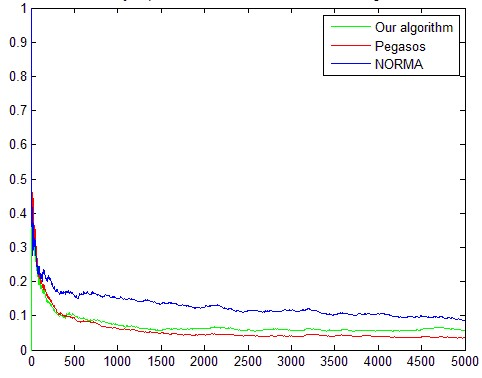
\includegraphics[width=0.9\linewidth]{PN_Lin_Lin}
\label{LL}
        \caption{Linearly separable dataset}
      \end{subfigure}%
\hspace{.01\linewidth}
\begin{subfigure}[b]{.45\linewidth}
	 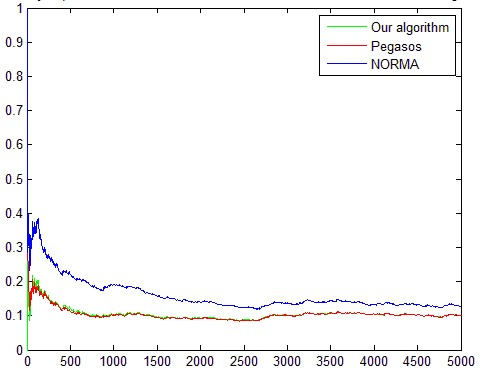
\includegraphics[width=0.9\linewidth]{PN_Noise_Lin.jpg}
       \label{NL}
      \caption{Linear dataset with noise}
  
	 \end{subfigure}%

 \begin{subfigure}[c]{.45\linewidth}
	   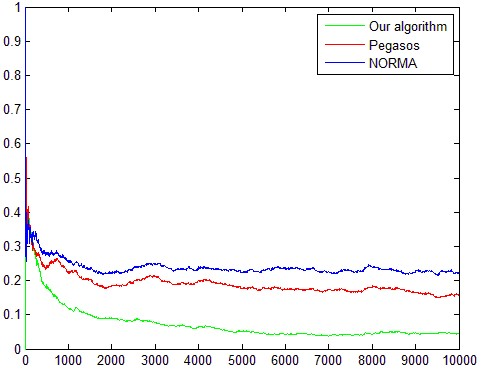
\includegraphics[width=0.9\linewidth]{PN_Bayess_Lin}
           \label{BL}
           \caption{Bayes-separable dataset with fixed distribution parameters}
 \end{subfigure}%
\hspace{.01\linewidth}
\begin{subfigure}[c]{.45\linewidth}
    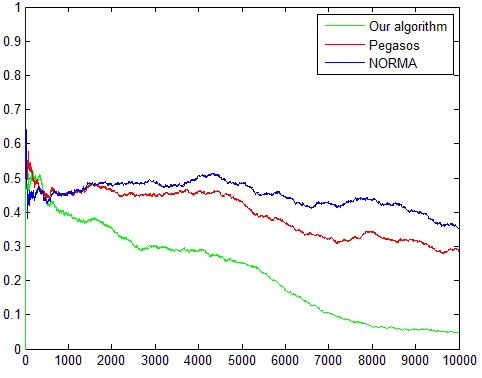
\includegraphics[width=0.9\linewidth]{PN_Move_Lin}
    \label{ML} 
   \caption{Bayes-separable dataset with drifting distribution parameters}
\end{subfigure}%

\begin{subfigure}[c]{.45\linewidth}
	   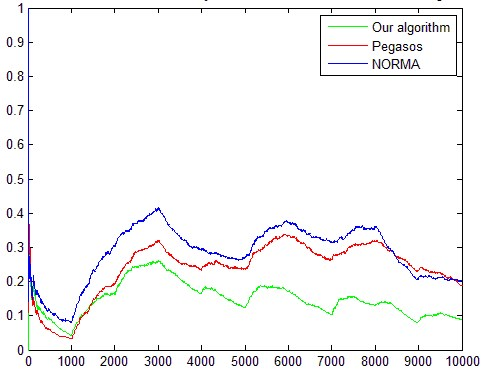
\includegraphics[width=0.9\linewidth]{PN_Switch_Lin}
\label{SL}
\caption{Bayes-separable dataset with parameters being switched every 1000 iterations}
\end{subfigure}%
\hspace{.01\linewidth}
\begin{subfigure}[c]{.45\linewidth}
	   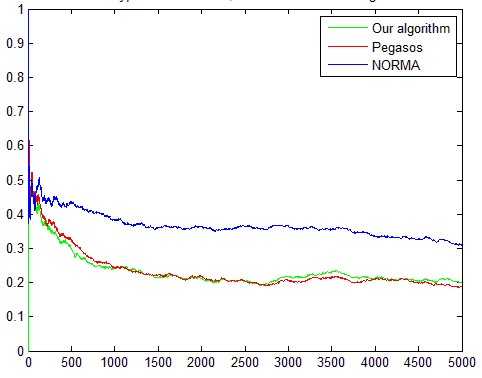
\includegraphics[width=0.9\linewidth]{PN_Cov_Lin}
\label{CtL}
\caption{ Covertype dataset}
\end{subfigure}%
    \caption{Experimental results comparing the performance of our algorithm to linear implementation of Pegasos and NORMA}
    \label{Result:LinearPN}
\end{figure*}

\begin{figure*}[t]
    \centering
\begin{subfigure}[b]{.45\linewidth}
       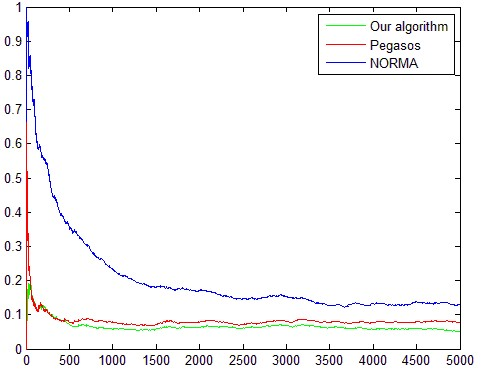
\includegraphics[width=0.9\linewidth]{PN_Lin_Gauss}
\label{LG}
        \caption{Linearly separable dataset}
      \end{subfigure}%
\hspace{.01\linewidth}
\begin{subfigure}[b]{.45\linewidth}
	 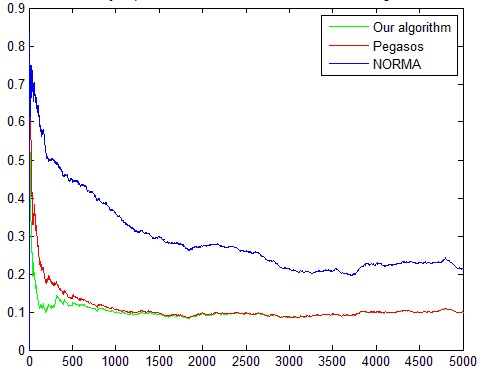
\includegraphics[width=0.9\linewidth]{PN_Noise_Gauss.jpg}
       \label{NG}
      \caption{Linear dataset with noise}
  
	 \end{subfigure}%

 \begin{subfigure}[c]{.45\linewidth}
	   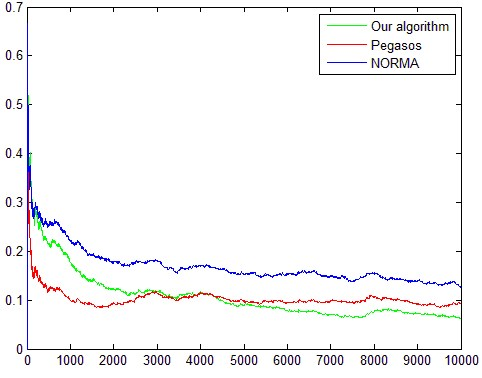
\includegraphics[width=0.9\linewidth]{PN_Bayess_Gauss}
           \label{BG}
           \caption{Bayes-separable dataset with fixed distribution parameters}
 \end{subfigure}%
\hspace{.01\linewidth}
\begin{subfigure}[c]{.45\linewidth}
    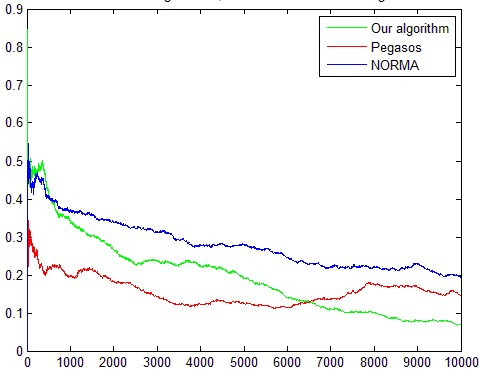
\includegraphics[width=0.9\linewidth]{PN_Move_Gauss}
    \label{MG} 
   \caption{Bayes-separable dataset with drifting distribution parameters}
\end{subfigure}%

\begin{subfigure}[c]{.45\linewidth}
	   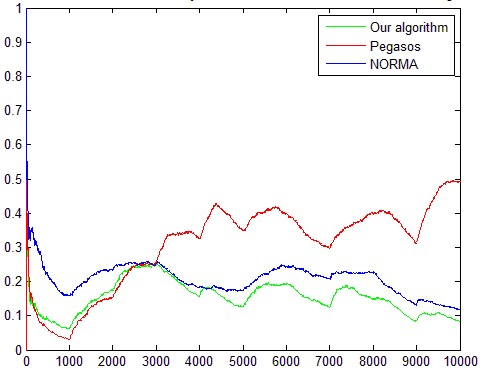
\includegraphics[width=0.9\linewidth]{PN_Switch_Gauss}
\label{SG}
\caption{Bayes-separable dataset with parameters being switched every 1000 iterations}
\end{subfigure}%
\hspace{.01\linewidth}
\begin{subfigure}[c]{.45\linewidth}
	   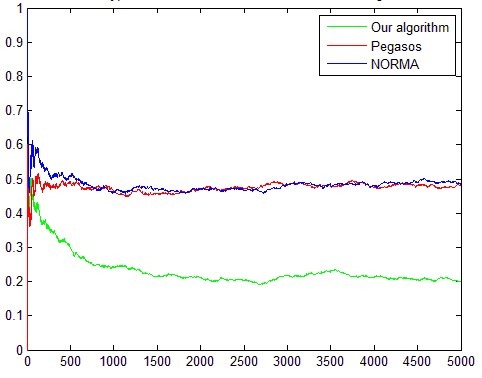
\includegraphics[width=0.9\linewidth]{PN_Cov_Gauss}
\label{CtG}
\caption{ Covertype dataset}
\end{subfigure}%
    \caption{Experimental results comparing the performance of our algorithm implementation of Pegasos and NORMA using Gaussian RBF}
    \label{Result:GaussPN}
\end{figure*}
\begin{table}
\centering
\begin{tabular}{| p{1.5cm}|  c |  c | c | c | c |}
\hline
 Dataset & O & PL & NL & PG & NG \\ \hline
Linear& 0.04 & 0.03 & 0.09 &0.07 &0.1 \\ \hline
Linear+ noise & 0.02 & 0.002 & 0.005 & 0.02 & 0.08 \\ \hline
Bayesian & 0.03 &0.17 & 0.22 & 0.08 & 0.15 \\ \hline
Drifting & 0.04 & 0.28 & 0.35 & 0.15&0.18 \\ \hline
Switching & 0.11 & 0.20 &0.21 & 0.32 & 0.13  \\ \hline
Covertype & 0.19 & 0.2 & 0.35 & 0.43 & 0.48 \\
\hline
\end{tabular}

\caption[Comparison to NORMA and Pegasos: Error rate over testing dataset]{Error rate over the testing dataset, O - our algorithm, PL -linear Pegasos, NL - linear NORMA, PG - Pegasos using Gaussian RBF kernel with $\gamma=0.01$, NG - NORMA with the same kernel}
\label{GenError}
\end{table}

\section{Comparison to offline algorithm: AdaBoost}
\label{AdaCompare}
In the interests of fairness, we also compare our algorithm to the AdaBoost in the offline setting. Since our algorithm is designed for online usage, we simulate the online environment by sequentially feeding it data samples randomly selected from the training dataset. Since a single iteration of the AdaBoost results in an additional weak classifier being added, while our algorithm takes $r$ iterations to do the same, to obtain equivalent conditions for testing we only evaluate the accuracy of our algorithm every $r$'s iteration. Also for equivalence, we use a pool of $M$ randomly selected linear classifiers for weak classifier selection.

It should be noted that the above condition does not mean that our algorithm is more computationally intensive, since to choose a classifier for addition the AdaBoost algorithm has to calculate weighted error rates of every classifier in the selection pool to select a maximum, or use some optimization algorithm to obtain best classifier in the case of continuous classifier pool, resulting, in the discrete case, in $MN$ classifier evaluations, where $N$ is the number of training samples. Our algorithm, however, only performs $rK$ evaluations,  with $r \ll N$ and $K$ being the number of classifiers already added.  In fact,  in the online case our algorithm is similar to AdaBoost evaluating on the random subset of the classifier pool on the random subset of training data. 
\begin{figure*}[t]
    \centering
\begin{subfigure}[b]{.45\linewidth}
       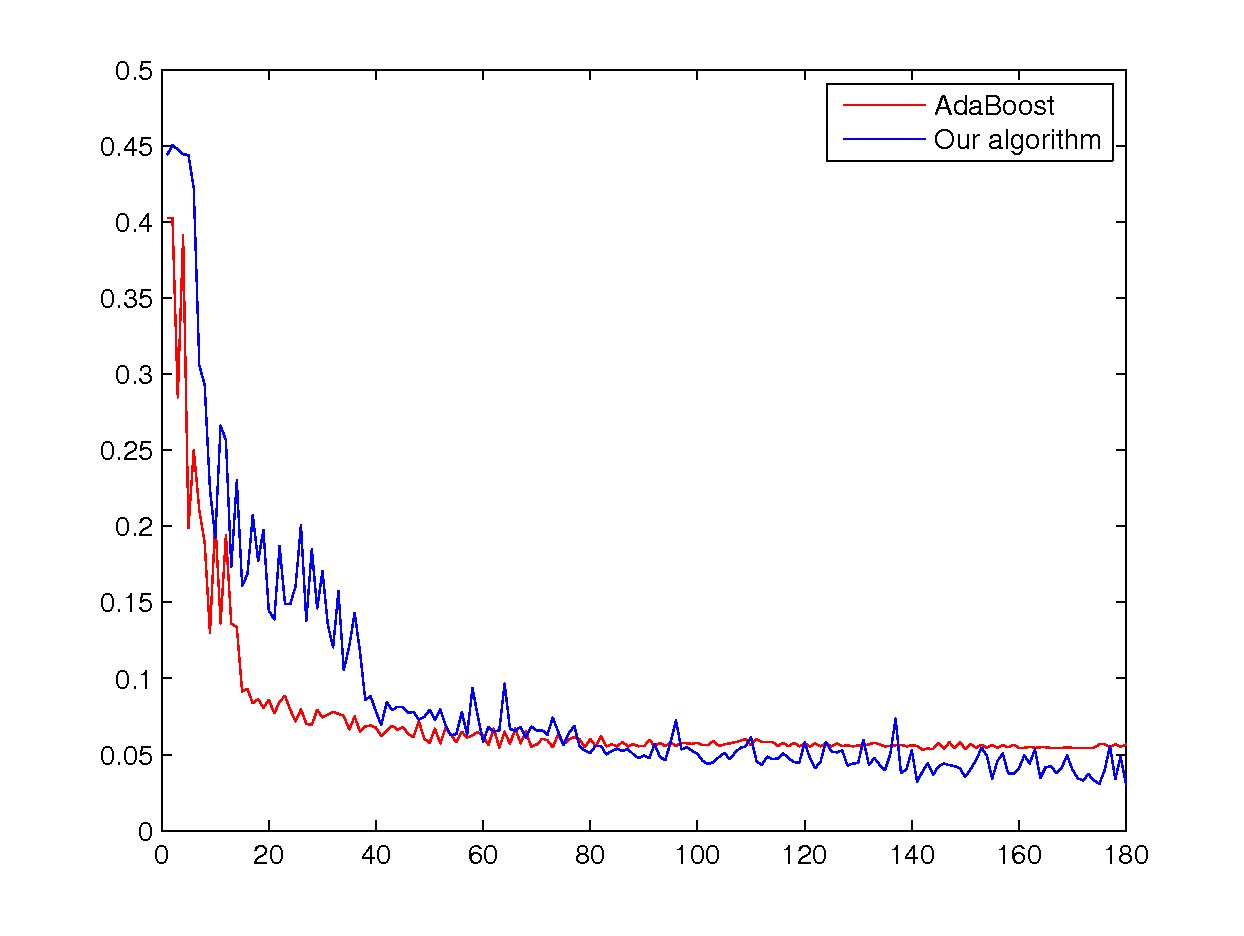
\includegraphics[width=0.9\linewidth]{adas}
\label{noref1}
        \caption{Synthetic nonlinear dataset}
      \end{subfigure}%
\hspace{.01\linewidth}
\begin{subfigure}[b]{.45\linewidth}
	 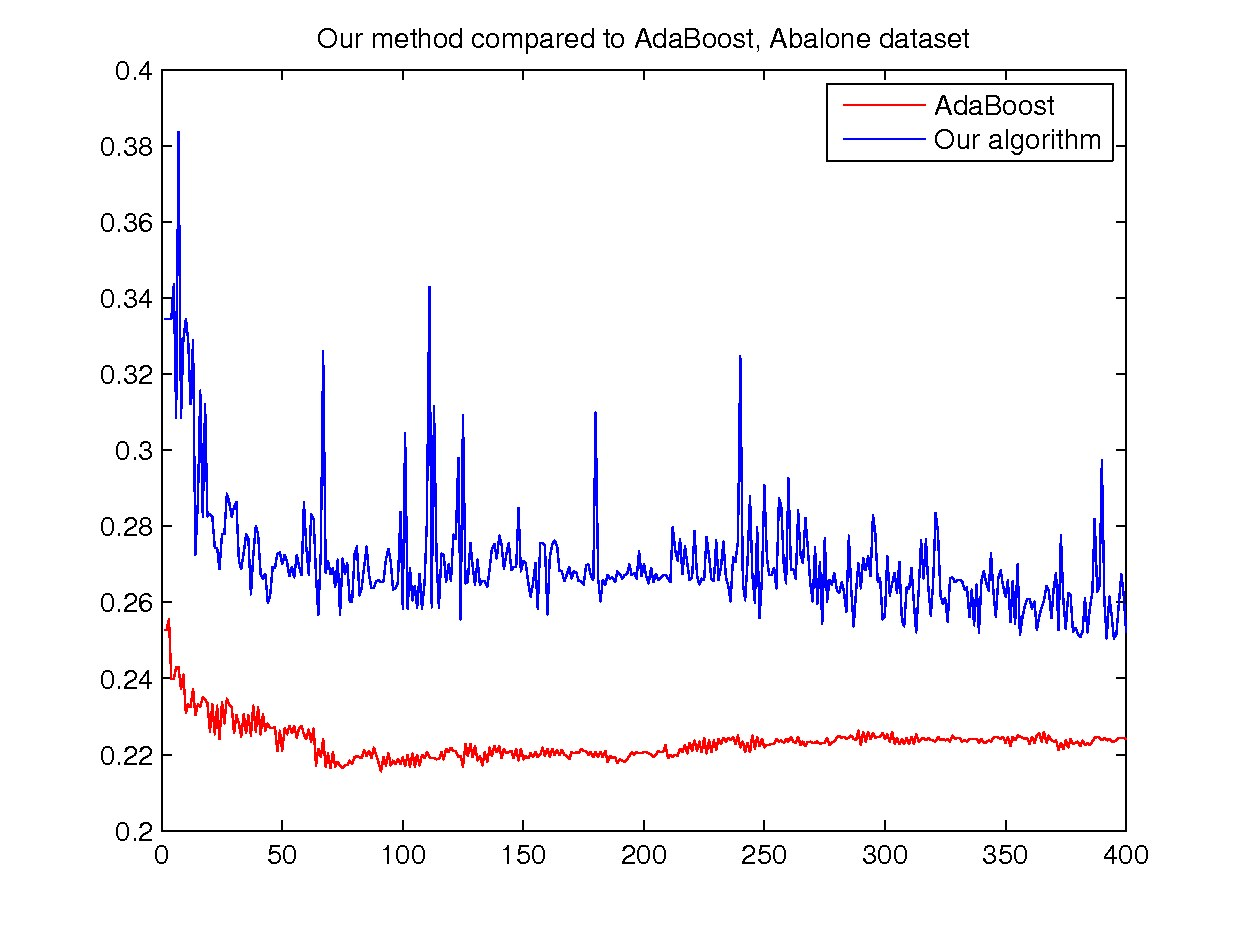
\includegraphics[width=0.9\linewidth]{adaab}
       \label{noref2}
      \caption{Abalone dataset}
  
	 \end{subfigure}%

    \caption{Experimental results comparing the performance of our algorithm to AdaBoost}
    \label{adacom}
\end{figure*}
We evaluate the methods on two datasets, one being a synthetic nonlinearly separable dataset, and the other  being the Abalone dataset from the UCI database (\cite{frafra}), with classes 10-29 merged into a positive class and other classes being negative. The results of generalized error on the number of classifiers added are presented on \figref{adacom}. They clearly show, that while on the offline setting AdaBoost outperforms our algorithm, the increase in the convergence speed is not very large. This advantage is due to the fact that our algorithm only selects near-optimal classifier on each addition, while AdaBoost uses the optimally selected one. 
\section{Comparison to the online AdaBoost}
\begin{figure}[t]
		\centering
		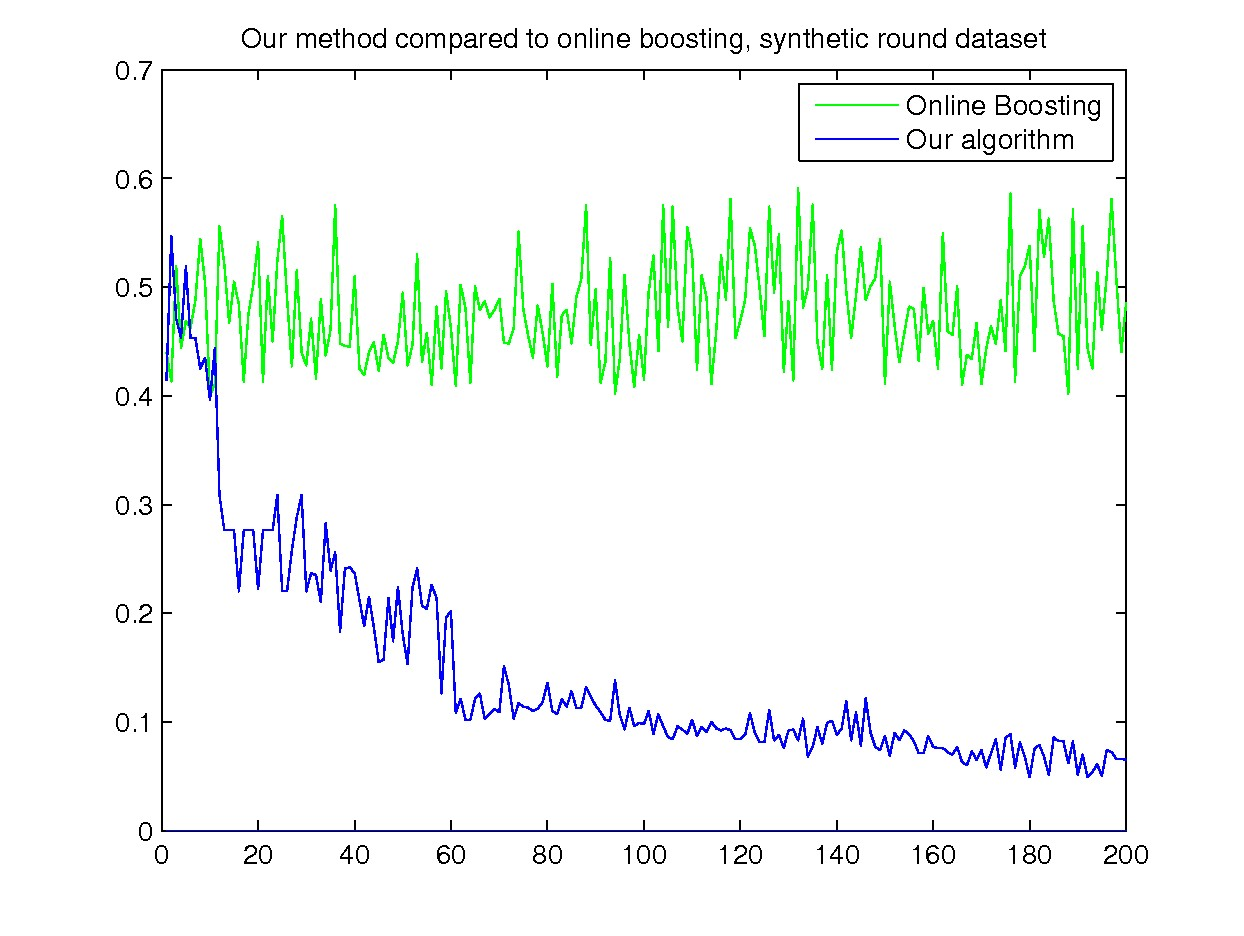
\includegraphics[width=0.7\textwidth]{odas}
		\caption{Experimental results comparing the performance of our algorithm to online boosting}
		\label{odacom}
	\end{figure}

We also compare our algorithm to the performance of the online AdaBoost presented in \cite{OnlineBoost}. We use the same datasets as in above section(\ref{AdaCompare}), with the difference being that the synthetic dataset is not pregenerated, since both of the algorithms are adapted to the online usage. 

For weak classifiers, we again use randomly generated linear classifiers, and for update stage of online Boosting algorithm we use the Pegasos iteration. 

The results of convergence experiments are shown on \figref{odacom}. They show that the online boosting algorithm underperforms compared to our algorithm, and is less stable. It does not converge well for both synthetic and Abalone dataset (not pictured).
It is also much more computationally expensive for the number of selectors equal to the number of classifiers added by our algorithm due to the fact that it performs updates on the whole pool of classifiers at once to estimate the optimal one. We can conclude that for most cases our algorithm would be superior to the online boosting.



% ---------------------------------------------------------------------------
%: ----------------------- end of thesis sub-document ------------------------
% ---------------------------------------------------------------------------



% this file is called up by thesis.tex
% content in this file will be fed into the main document

\chapter{Conclusion} % top level followed by section, subsection

The main goal of the work presented in this thesis is development of the new online methods, and proving its applicability to the real-world tasks in image processing. After reviewing the state-of-the art methods, including online SVM training and boosting, we have developed our own method combining  effectiveness of the offline AdaBoost and convergence properties of the online methods like Pegasos. We have proposed a methods iteratively adding and training weak classifiers while at the same time updating the boosting coefficients combining them into a strong classifier with increased accuracy. The resulting algorithm can be used for both linear and non-linear classification, and exhibits high stability in regard to improperly tuned parameter, allowing to use the same parameter set for varying data distribution. Furthermore, it has lower computational and memory requirements than the the state-of-the art methods it was derived from. 
To show the effectiveness of the proposed algorithms have evaluated our method against Pegasos (\cite{Pegasos}), NORMA  (\cite{Norma}) and online boosting (\cite{OnlineBoost}), all methods quite popular in the scientific community for use with large datasets. We used several synthetic and publicly available natural datasets to show the stability and improved convergence rate of our method compared to other methods.

To further show the practical applicability of our algorithm, we have developed a simple tracking application for the mobile device that uses our learning method to learn and maintain object model. We have introduced a set of simple features sufficient to identify certain classes of object, and have shown that our method allows their combination into a relatively stable tracker that runs at near real-time speed (12-15 fps) even with unoptimized code. This application, then serves as a proof-of-concept application demonstrating the utility of our learning technique.


% ----------------------- paths to graphics ------------------------

% change according to folder and file names
\ifpdf
    \graphicspath{{7/figures/PNG/}{7/figures/PDF/}{7/figures/}}
\else
    \graphicspath{{7/figures/EPS/}{7/figures/}}
\fi


% ----------------------- contents from here ------------------------






% ---------------------------------------------------------------------------
% ----------------------- end of thesis sub-document ------------------------
% ---------------------------------------------------------------------------               % discussion of results




% --------------------------------------------------------------
%:                  BACK MATTER: appendices, refs,..
% --------------------------------------------------------------

% the back matter: appendix and references close the thesis


%: ----------------------- bibliography ------------------------

% The section below defines how references are listed and formatted
% The default below is 2 columns, small font, complete author names.
% Entries are also linked back to the page number in the text and to external URL if provided in the BibTex file.

% PhDbiblio-url2 = names small caps, title bold & hyperlinked, link to page 
\begin{multicols}{2} % \begin{multicols}{ # columns}[ header text][ space]
\begin{tiny} % tiny(5) < scriptsize(7) < footnotesize(8) < small (9)

\bibliographystyle{Latex/Classes/PhDbiblio-url2} % Title is link if provided
\renewcommand{\bibname}{References} % changes the header; default: Bibliography

\bibliography{9_backmatter/references} % adjust this to fit your BibTex file

\end{tiny}
\end{multicols}

% --------------------------------------------------------------
% Various bibliography styles exit. Replace above style as desired.

% in-text refs: (1) (1; 2)
% ref list: alphabetical; author(s) in small caps; initials last name; page(s)
%\bibliographystyle{Latex/Classes/PhDbiblio-case} % title forced lower case
%\bibliographystyle{Latex/Classes/PhDbiblio-bold} % title as in bibtex but bold
%\bibliographystyle{Latex/Classes/PhDbiblio-url} % bold + www link if provided

%\bibliographystyle{Latex/Classes/jmb} % calls style file jmb.bst
% in-text refs: author (year) without brackets
% ref list: alphabetical; author(s) in normal font; last name, initials; page(s)

%\bibliographystyle{plainnat} % calls style file plainnat.bst
% in-text refs: author (year) without brackets
% (this works with package natbib)


% --------------------------------------------------------------

% according to Dresden med fac summary has to be at the end
%
% Thesis Abstract -----------------------------------------------------


%\begin{abstractslong}    %uncommenting this line, gives a different abstract heading
\begin{abstracts}        %this creates the heading for the abstract page

We describe and analyze a simple and effective two-step online boosting algorithm that allows us to utilize highly effective stochastic gradient descent based methods developed for online SVM training without the need to fine-tune kernel parameters, and show its efficiency by several experiments. Our method is similar to the AdaBoost in that it trains additional classifiers according to the weights provided by previously trained classifiers, but unlike AdaBoost we utilize hinge loss rather than exponential loss, and modify algorithm for online setting, allowing for varying number of classifiers. 
We show the effectiveness of our method by developing applying it to the task of object tracking on the mobile device (iPhone). In order to achieve the real-time processing speed we furthermore describe a set of compact features in order to fully utilize the parallel processing capabilities of the device GPU. We then show that utilizing our algorithm with such features allows for a high discrimination rate even with a small number of features being utilized.


\end{abstracts}
%\end{abstractlongs}


% ---------------------------------------------------------------------- 


%: Declaration of originality
%
% Thesis statement of originality -------------------------------------

% Depending on the regulations of your faculty you may need a declaration like the one below. This specific one is from the medical faculty of the university of Dresden.

\begin{declaration}        %this creates the heading for the declaration page

I herewith declare that I have produced this paper without the prohibited assistance of third parties and without making use of aids other than those specified; notions taken over directly or indirectly from other sources have been identified as such. This paper has not previously been presented in identical or similar form to any other Japanese or foreign examination board.

The thesis work was conducted from April, 2007 to July 2012 under the supervision of Prof. Itsuo Kumazawa at Tokyo Institute of Technology.

\vspace{10mm}

Tokyo, 2012


\end{declaration}


% ----------------------------------------------------------------------



\end{document}
